% Plant Physiology submission version of main.tex (built by make_plantphys.py).
% Edit main.tex as the source of truth, or edit this file directly if you prefer;
% the two are not kept in sync automatically.
% Compile from final/plant_physiology/:  pdflatex, bibtex, pdflatex, pdflatex
\documentclass[namedate,unnumsec,webpdf,contemporary,large]{oup-authoring-template}
\usepackage{tabularx}
\usepackage{microtype}
% let TeX stretch spaces instead of pushing long gene IDs into the margin
\setlength{\emergencystretch}{3em}
\usepackage{booktabs}
\newcolumntype{b}{X}
\newcolumntype{s}{>{\hsize=.5\hsize}X}
\newcommand{\societylogo}{}

\begin{document}

\journaltitle{Plant Physiology}
\DOI{DOI added during production}
\copyrightyear{2026}
\pubyear{2026}
\access{Advance Access Publication Date: Day Month Year}
\appnotes{Research Article}
\firstpage{1}

\title[Aspartate pathway and maize grain nitrogen]{The aspartate-to-homoserine pathway recurs across maize grain amino acids, soil nitrogen, and yield selection}

\author[1,$\dagger$]{Nirwan Tandukar}
\author[2,3,$\dagger$]{Sarah Fitzsimmons}
\author[4,1]{Sherry Flint-Garcia}
\author[2,5]{Ruthie Angelovici}
\author[1,$\ast$]{Rub\'en Rell\'an-\'Alvarez}

\address[1]{\orgdiv{Department of Molecular and Structural Biochemistry, N.C. Plant Sciences Initiative, Genetics and Genomics Program}, \orgname{North Carolina State University}, \orgaddress{\state{Raleigh, NC}, \country{USA}}}
\address[2]{\orgdiv{Division of Biological Sciences}, \orgname{University of Missouri}, \orgaddress{\state{Columbia, MO 65211}, \country{USA}}}
\address[3]{\orgdiv{Department of Agronomy and Plant Genetics}, \orgname{University of Minnesota}, \orgaddress{\state{St. Paul, MN}, \country{USA}}}
\address[4]{\orgname{USDA-ARS Plant Genetics Research Unit}, \orgaddress{\state{Columbia, MO 65211}, \country{USA}}}
\address[5]{\orgdiv{Department of Plant Biology}, \orgname{Michigan State University}, \orgaddress{\state{East Lansing, MI}, \country{USA}}}

\corresp[$\dagger$]{These authors contributed equally to this work. $^{\ast}$Corresponding authors. Sherry Flint-Garcia (\href{mailto:sherry.flint-garcia@usda.gov}{sherry.flint-garcia@usda.gov}), Ruthie Angelovici (\href{mailto:angelovicir@missouri.edu}{angelovicir@missouri.edu}), and Rub\'en Rell\'an-\'Alvarez (\href{mailto:rrellan@ncsu.edu}{rrellan@ncsu.edu})}

\abstract{Grain nitrogen (N) in maize depends on N uptake, assimilation, and allocation, but it is unclear whether the same metabolic functions underlie natural variation in grain amino acid composition, genetic variation associated with soil N, and response to selection. We tested this in three populations, each with a distinct N-related phenotype. In the Goodman--Buckler Association Panel, grain free amino acids were dominated by asparagine and proline and were highly heritable, and genome-wide association mapping of 71 traits implicated genes for amino acid metabolism and transport. The loci shared across the most traits lay near a peptidase A1 gene and endoplasmic reticulum membrane protein genes. In 3,107 georeferenced landraces from across the Americas, association mapping of soil N at collection sites identified variants near an aspartate kinase isozyme and an omega-amidase that passed tests for confounding with geography and climate. Indian Chief and Jarvis responded to 14 cycles of reciprocal recurrent selection for yield with different changes in N allocation. The two populations diverged genetically, and Indian Chief accumulated more free amino acids, mostly proline, while protein-bound amino acids were unchanged. Their candidate regions included protein-turnover genes in Indian Chief and amino acid importers in Jarvis, consistent with these population-specific phenotypes. Each of the four analyses highlighted a different enzyme of the aspartate-to-homoserine pathway, the only pathway that remained significant after correction across all pathways. Together, these results point to aspartate-family metabolism as a shared source of candidate genes for how N is partitioned among grain amino acid pools in maize.}

\keywords{maize, grain nitrogen, free amino acids, aspartate-family amino acids, genome-wide association, reciprocal recurrent selection}

\maketitle

\section{Introduction}

Nitrogen (N) is essential for maize growth and kernel development, but its use in agriculture is a major sustainability challenge. Crop production relies heavily on N fertilizer, yet much of the applied N is not recovered by the crop and is lost through leaching, runoff, or gaseous emissions \citep{OjedaRivera2025NitrogenEfficientMaize}. Reducing these losses requires understanding how plants acquire, assimilate, transport, and remobilize N, and how they allocate it to the developing grain \citep{MasclauxDaubresse2010NUE,Have2017NRemobilization}. In maize kernels, N is held in free amino acids (FAAs) and protein-bound amino acids (PBAAs), so grain amino acid composition is a direct biochemical readout of how N is allocated to the grain.

Plant N metabolism centers on a few key amino acids. Ammonium is assimilated via the GS/GOGAT cycle, producing glutamine and regenerating glutamate from 2-oxoglutarate, so Glu/Gln metabolism links N assimilation with carbon metabolism \citep{MasclauxDaubresse2010NUE,Hodges2002TwoOxoglutarate}. Glutamine and asparagine are the main N-rich transport and storage forms, while glutamate and aspartate donate amino groups to carbon skeletons \citep{Bernard2009CytosolicGS,MasclauxDaubresse2010NUE}. Aspartate is particularly important because it feeds asparagine and the aspartate-family amino acids (methionine, threonine, lysine, isoleucine) \citep{Viola2001AspartatePathway, Wang2018AspSeeds, Han2021Aspartate}. During grain filling, protein degradation in senescing leaves releases amino acids that supply grain N \citep{Have2017NRemobilization, Liu2008ProteinDegradationNRemobilization}. Proline adds a stress-related component, with genotype-dependent accumulation and export from maize leaves under water stress \citep{Carceller1999ProlineRemobilization}. Thus, shifts in grain FAA composition may reflect redistribution among multiple N pools, not just changes in total N.

Most grain N is stored in storage proteins, so protein-bound amino acid composition is largely determined by the proteins produced. The free amino acid pool is small but reflects amino acids delivered to and metabolized in the developing kernel, and may therefore better indicate N supply. How much this pool varies heritably among lines, and which genes control that variation, is less well known than for protein-bound amino acids \citep{Shrestha2022}.

Maize germplasm enables grain N metabolism to be studied in three ways. First, standing variation among inbred lines. The Goodman--Buckler panel captures much of the allelic diversity in public breeding and has been used to map grain composition traits \citep{FlintGarcia2005Goodman,Shrestha2022}. Second, adaptation to soil. The landraces evolved under local conditions across the Americas, so alleles affecting N acquisition or use may correlate with soil N at collection sites. Georeferenced landraces enable environmental GWAS \citep{RomeroNavarro2017Landraces}, but soil N covaries with geography and climate and must be controlled. Third, selection for yield. Fourteen cycles of reciprocal recurrent selection in Indian Chief and Jarvis altered N uptake and allocation \citep{Comstock1949RRS,MollStuber1971}. Jarvis increased grain N via post-anthesis uptake, while Indian Chief retained more N in stover \citep{Moll1994}. Comparing Cycle 0 vs. Cycle 14 highlights regions with large allele-frequency shifts, though drift is also substantial in small populations \citep{Gerke2015DriftRRS}.

These populations differ in germplasm, in the N-related phenotype measured, and in how genetic signals are detected, so the same genes are not expected to appear in all of them. Each analysis also yields hundreds to thousands of candidate genes, many of which overlap by chance. If N metabolism shapes all three, however, different genes in the same metabolic pathways could be implicated. We therefore compared the analyses at the pathway level, asking whether any pathway contained candidates from more analyses than expected by chance.

We combined grain amino acid profiling and GWAS in the Goodman--Buckler panel, soil-N environmental GWAS in landraces, genomic population scans of Indian Chief and Jarvis, and reanalyzed the B64 $\times$ CML14 biparental population developed for grain asparagine variation for aspartate and proline. We analyzed free and protein-bound amino acid pools, focusing on asparagine, aspartate, glutamate, glutamine, and proline because of their roles in N transport, C--N metabolism, and storage. Although candidate regions overlapped no more than expected by chance, each analysis implicated a different enzyme of the aspartate-to-homoserine pathway, the only pathway that remained significant after correction. Beyond this pathway, individual candidates pointed to the aspartate--glutamate junction, where amino acid N connects with C--N recycling, and to amino acid transport and protein turnover, with different functions highlighted in each population. Together, these results suggest that aspartate-family metabolism is a shared source of variation in maize N metabolism.

\section{Results}

\subsection{Kernel free amino acid composition in the Goodman--Buckler panel is dominated by asparagine and proline}

FAA composition was evaluated across 280 of the 282 lines in the Goodman--Buckler panel grown in four replicates (two years $\times$ two blocks, Supplemental Tables S1--S2). Asn and Pro were the most abundant amino acids. Asn ranked first in 146 genotypes (52\%) and Pro in 118 (42\%), and the two were the top amino acids in 179 of 280 genotypes (64\%, Supplemental Figure~S1A--B). Asn was about 144 times as abundant as Cys (Supplemental Figure~S1C), but abundance did not predict variability among lines. Met varied the most (coefficient of variation, CV, 180\%), while Glu, Trp, and Gly varied the least (CV 44--54\%, Supplemental Table S3).

Differences among lines were consistent across years. For the 251 lines grown in both years, line means were correlated between years for all free amino acids (Spearman $\rho = 0.33$--0.75, median 0.56, Supplemental Table S3). Median broad-sense heritability ($H^2$) was 0.75 for the 20 FAAs (0.47--0.88), compared with 0.60 for the 15 PBAAs measured by \citet{Shrestha2022}, and was highest for Lys (0.88), Asn (0.83), Asp (0.81), and Pro (0.80). Median genomic heritability ($h^2$) was 0.48 for FAAs and 0.34 for PBAAs (Supplemental Figure~S2, Supplemental Table S4).

The protein-bound pool dominated grain amino acids, exceeding the free pool 47-fold for total amino acids and 42-fold for amino acid-derived N (paired Wilcoxon tests, all $P < 10^{-40}$, Supplemental Figure~S3, Supplemental Table S5), so FAAs contributed only 2.4\% of grain amino acid-derived N. However, composition differed between the pools. Pro made up 23.1\% of FAAs but 10.6\% of PBAAs, and its fraction varied far more among lines in the free pool (CV 44\% compared with 8\%). Thus, the free pool is small but variable and reproducible among lines, which makes it suitable for association mapping.

%===================== FIGURE 1 =====================

\begin{figure*}[ht!]
    \centering
    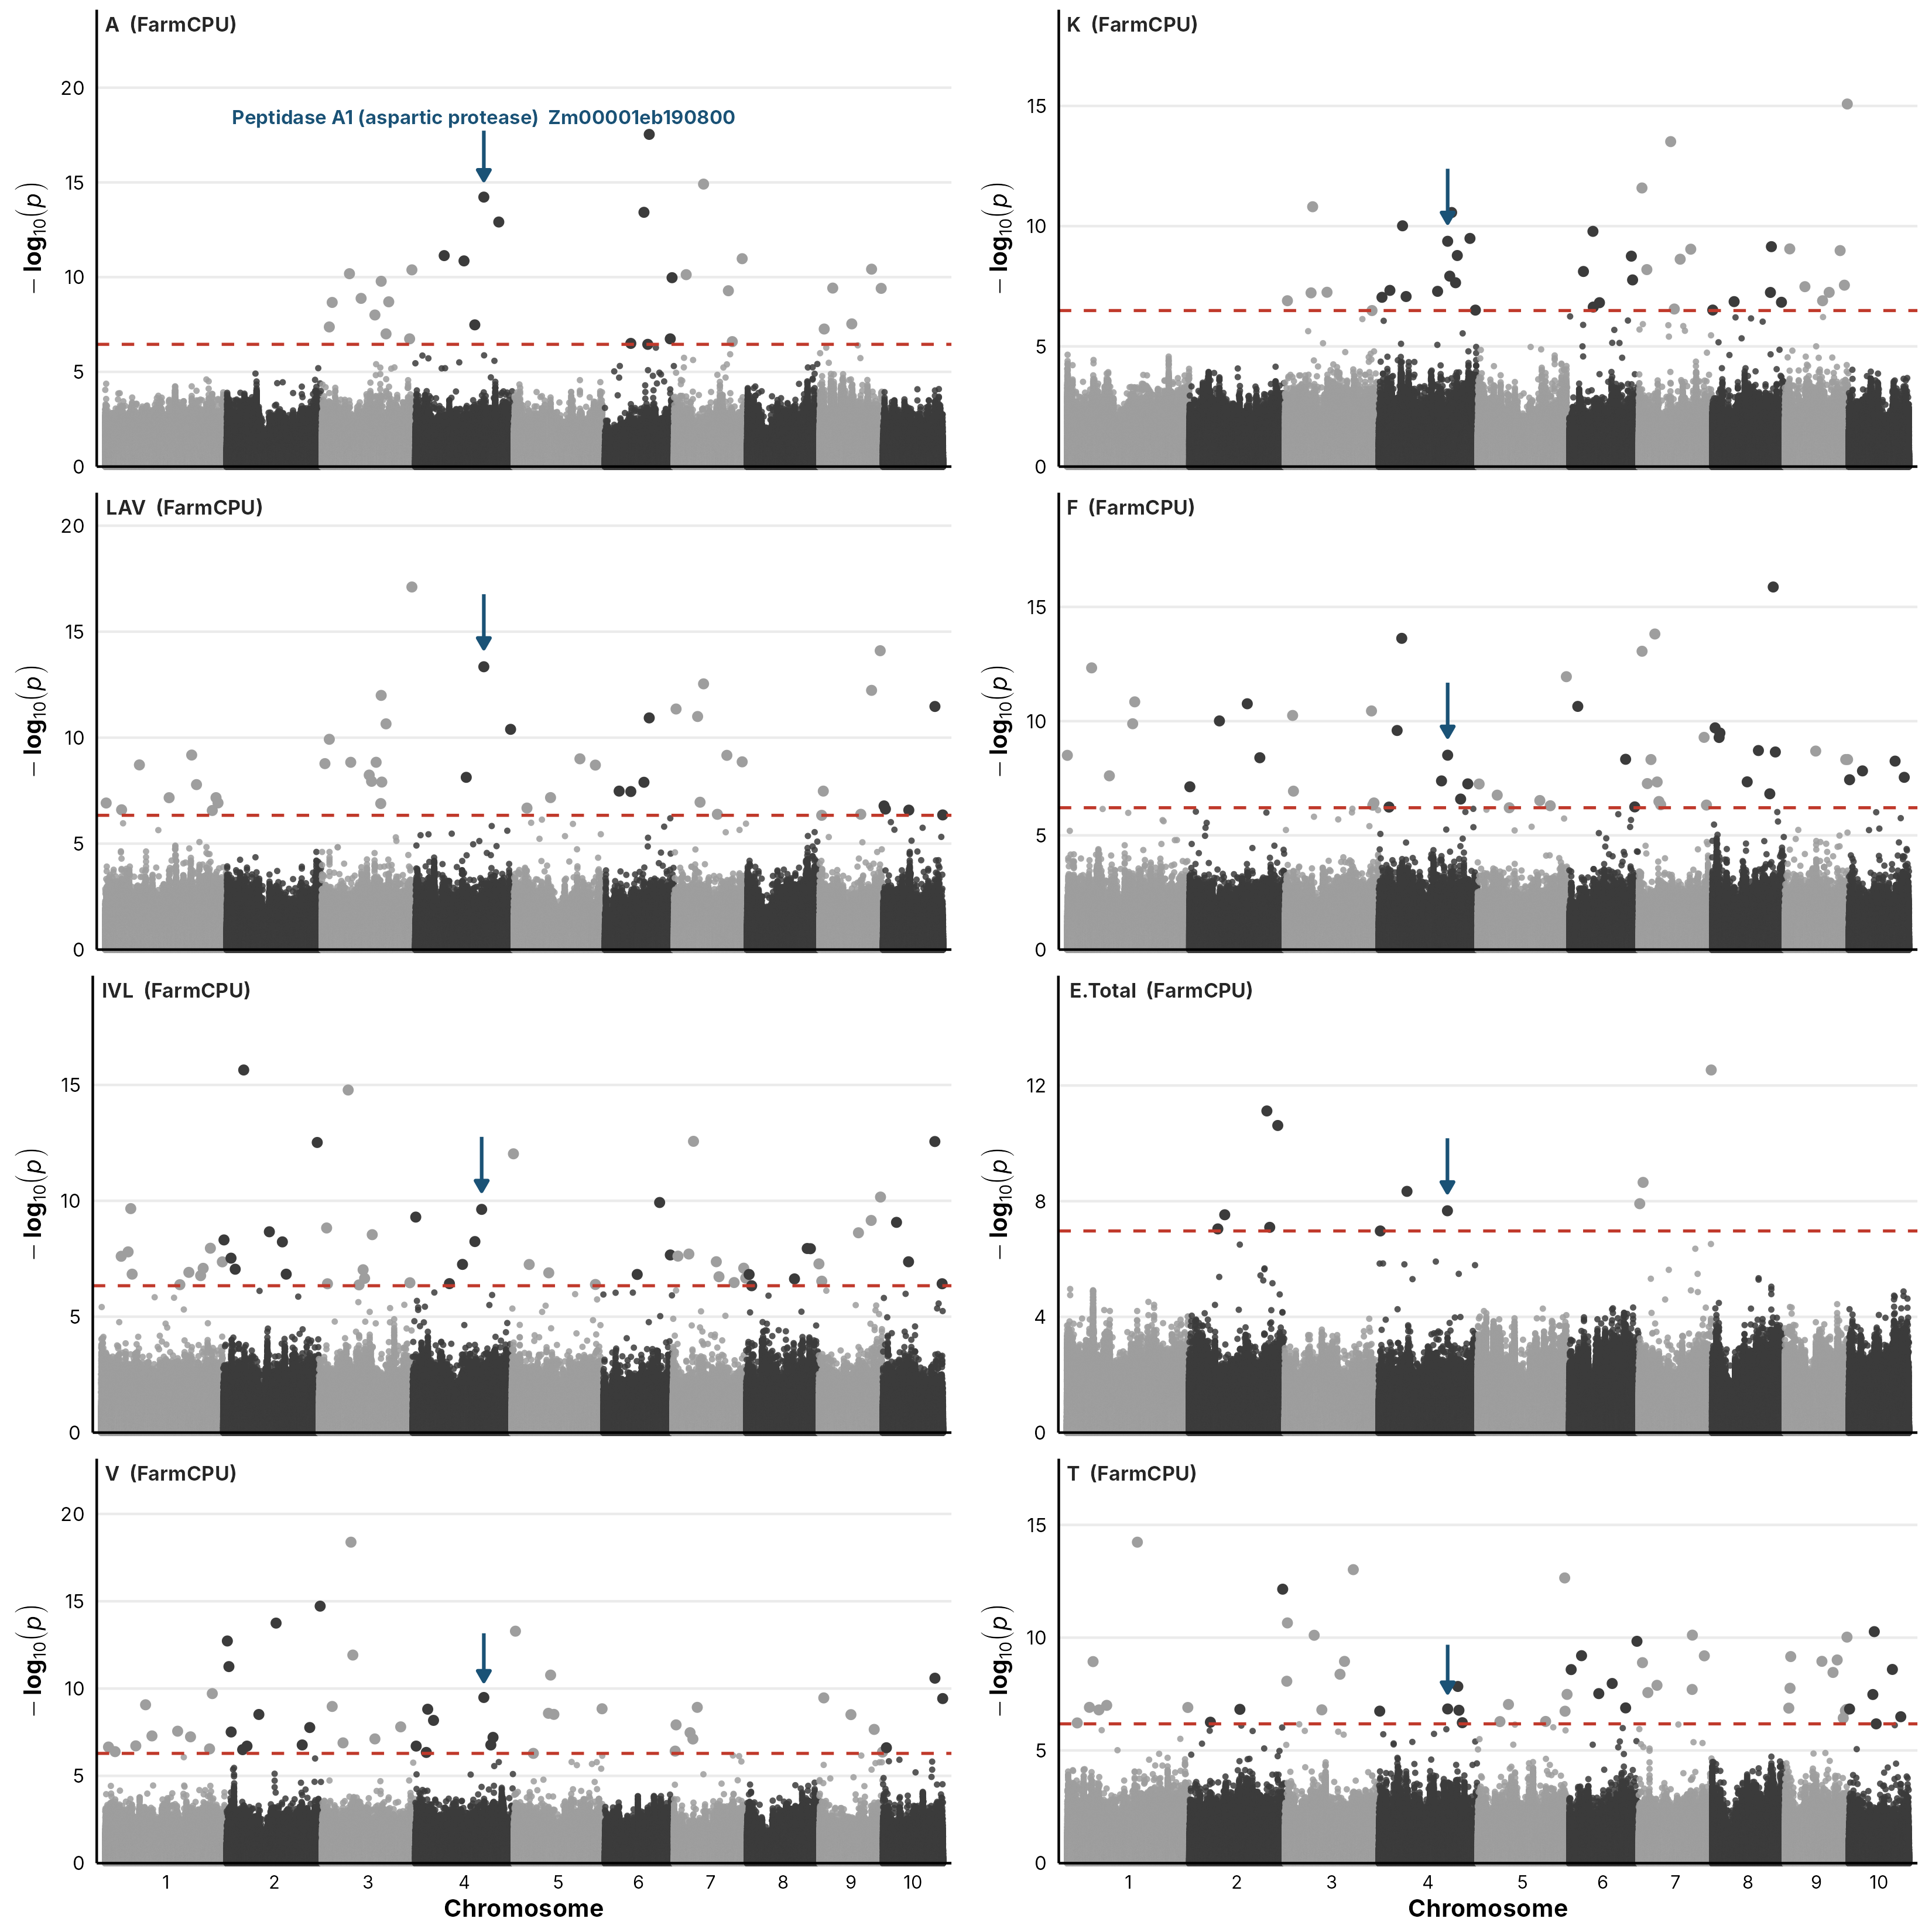
\includegraphics[width=0.82\textwidth]{figures/Fig_amino_chr4_peptidaseA1_manhattan.png}
    \caption{\textbf{Manhattan plots associated with eight amino acid traits link to an aspartic protease gene} A chromosome 4 locus associated with alanine (\textit{A}), \textit{LAV}, \textit{IVL}, valine (\textit{V}), lysine (\textit{K}), phenylalanine (\textit{F}), \textit{E.Total}, and threonine (\textit{T}) lies adjacent to a peptidase A1 (aspartic protease) gene. FarmCPU Manhattan plots show the significant traits at chr4:174.55–174.57 Mb. Arrows indicate the top SNP within \textit{Zm00001eb190800}. Red dashed lines mark the 5\% Benjamini–Hochberg FDR thresholds.}
    \label{fig:amino_locus_manhattan}
% Alt text: TODO (required by Plant Physiology for each figure)
\end{figure*}

\subsection{Association mapping identifies amino acid metabolism and transport candidates for abundant, heritable free amino acids}

We ran GWAS for 78 amino acid phenotypes (Supplemental Table S2) with three models (MLM, BLINK, and FarmCPU). At a Benjamini--Hochberg FDR of 5\%, 2,461 SNPs were significant for at least one of 71 phenotypes. Significant SNPs within 25~kb of each other identified 2,152 loci and 3,693 candidate genes (Supplemental Tables S6--S7). Most candidate genes were specific to one phenotype (3,002), and only 193 were shared by more than two. A locus on chromosome 9 (133.93 Mb) associated with nine phenotypes contained an ER membrane protein complex subunit 4 gene (\textit{Zm00001eb394360}) and a rhomboid-like protein gene (\textit{Zm00001eb394380}), but its phenotypes were explained by only three groups of SNPs (Supplemental Figure~S4), because many phenotypes are ratios or composites of the same amino acids. A locus on chromosome 4 at 174.57 Mb was associated with eight phenotypes from four biosynthetic families (\textit{A}, \textit{V}, \textit{K}, \textit{F}, \textit{T}, \textit{LAV}, \textit{IVL}, and \textit{E.Total}), with significant SNPs 2.6--6.1 kb upstream and 5.9~kb downstream of a peptidase A1 (aspartic protease) gene (\textit{Zm00001eb190800}, Figure~\ref{fig:amino_locus_manhattan}).

Among individual FAAs (Table~\ref{tab:amino_gwas_focus}), Asn had the most loci (356 across abundance and five ratios), with candidates including homoserine dehydrogenase (\textit{Zm00001eb405410}, \textit{N.IMNTDK}, SNP within the gene), two asparagine synthetase domain genes (\textit{Zm00001eb036060}, \textit{Zm00001eb036070}), the Lys-branch enzymes dihydrodipicolinate synthase and reductase (\textit{Zm00001eb389290}, \textit{Zm00001eb176170}), and the vacuolar transporter AVT6C (\textit{Zm00001eb368680}), which was significant for Asn ($P = 1.3\times10^{-8}$) and the Asp-family composite in both BLINK and FarmCPU. A SNP for Lys as a fraction of the total free pool (\textit{K.Total}, $P = 2.5\times10^{-11}$) lies in the NRT1/PTR family 4.6 transporter gene \textit{Zm00001eb277160}. Pro had a lower genomic heritability than Asn ($h^2 = 0.40$ compared with 0.68) and fewer loci (59), and one Pro SNP lies within a class I glutamine amidotransferase gene (\textit{Zm00001eb217220}, $P = 2.2\times10^{-9}$). Gln had the strongest association among these amino acids (\textit{Q.E}, $P = 4.9\times10^{-22}$). A SNP for free Gln lies within a WAT1-related (UmamiT) gene (\textit{Zm00001eb379220}), and a SNP for the Gln/Glu ratio lies within the amino acid permease \textit{aaap40} (\textit{Zm00001eb261470}), in a region that also contains \textit{LHT1} and \textit{LHT2}. Met, the most variable FAA, had 104 loci but no trait-matched candidate gene. Thus, genes of Asn and Asp-family metabolism and amino acid transport were linked to individual amino acids, whereas loci shared by many phenotypes pointed to protein turnover and membrane protein biogenesis rather than single biosynthetic steps.

To test whether free Asp and Pro variation also segregates in a biparental cross, we mapped both traits in a B64 $\times$ CML14 F$_{2:3}$ population developed to map kernel free Asn \citep{Fitzsimmons2026KernelKitchen}. Because the parents were chosen for Asn, this analysis was exploratory (Supplemental Figure~S5A,C). Both traits mapped to the same position on chromosome 3 (peak at 35.99~Mb), with LOD 6.12 for Asp (threshold 3.70) and 4.55 for Pro (threshold 3.63), explaining 10\% and 7\% of phenotypic variance (Supplemental Figure~S5B,D). This shared QTL was distinct from the Asn QTL at \textit{ASN3} on chromosome~1. Its support interval spans the low-recombination region around the centromere and contains more than 1,500 genes (Supplemental Table S8), so it cannot resolve a causal gene. Within 1.5~cM of the peak, it does, however, include the tandem CC-type glutaredoxin genes (\textit{Zm00001eb131830}, \textit{Zm00001eb131840}) and an LHT-like amino acid transporter (\textit{Zm00001eb132750}), all of which also lie in highly differentiated Jarvis windows explained below.

%===================== TABLE 1 =====================

\begin{table*}[t]
\centering
\caption{\textbf{Association mapping of the focal FAAs in the Goodman--Buckler panel.} Median, coefficient of variation (CV), line-mean broad-sense heritability ($H^2$) and genomic heritability ($h^2_g$) are from Supplemental Table~S3. Loci: loci (Supplemental Table~S7) significant at 5\% Benjamini--Hochberg FDR for at least one phenotype reporting on the amino acid; in parentheses, loci for the absolute trait alone. Best $P$: smallest $P$ among those phenotypes. Trait-matched candidate genes: genes within 25 kb of a significant SNP with their putative function.}
\label{tab:amino_gwas_focus}
\footnotesize
\setlength{\tabcolsep}{3pt}
\begin{tabularx}{\textwidth}{@{}l r r r r r r >{\raggedright\arraybackslash}X@{}}
\hline
FAA & Median & CV (\%) & $H^2$ & $h^2_g$ & Loci & Best $P$ & Trait-matched candidate genes (putative function) \\
\hline
Asparagine (N) & 3.783 & 70 & 0.83 & 0.68 & 356 (73) & $2.8\times10^{-20}$ & \textit{Zm00001eb368680} (amino acid transporter AVT6C); \textit{Zm00001eb329710} (glutamine amidotransferase type 2); \textit{Zm00001eb405410} (homoserine dehydrogenase); \textit{Zm00001eb036060} (asparagine synthetase domain); \textit{Zm00001eb036070} (asparagine synthetase domain); \textit{Zm00001eb389290} (dihydrodipicolinate synthase); \textit{Zm00001eb176170} (dihydrodipicolinate reductase) \\
Proline (P) & 3.202 & 63 & 0.80 & 0.40 & 59 (59) & $2.7\times10^{-15}$ & \textit{Zm00001eb217220} (glutamine amidotransferase) \\
Lysine (K) & 0.272 & 90 & 0.88 & 0.73 & 116 (54) & $8.3\times10^{-16}$ & \textit{Zm00001eb277160} (NRT1/PTR family 4.6); \textit{Zm00001eb360480} (glutamate synthase (NADH)); \textit{Zm00001eb352400} (WAT1-related (UmamiT)) \\
Aspartate (D) & 1.178 & 76 & 0.81 & 0.84 & 91 (20) & $3.3\times10^{-16}$ & \textit{Zm00001eb207630} (WAT1-related (UmamiT)) \\
Glutamine (Q) & 0.371 & 130 & 0.69 & 0.85 & 165 (65) & $4.9\times10^{-22}$ & \textit{Zm00001eb379220} (WAT1-related (UmamiT)); \textit{Zm00001eb261470} (amino acid transporter); \textit{Zm00001eb261480} (amino acid transporter); \textit{Zm00001eb261490} (amino acid transporter) \\
Methionine (M) & 0.047 & 180 & 0.78 & 0.46 & 104 (56) & $3.2\times10^{-17}$ & none \\
\hline
\end{tabularx}
\end{table*}

\subsection{Soil nitrogen environment GWAS of maize landraces points to candidate genes in aspartate-family and amide nitrogen metabolism}

We next asked whether genetic variation associated with soil N implicates similar N-metabolism functions. We associated 3,107 georeferenced landraces \citep{RomeroNavarro2017Landraces} with soil N at their collection sites \citep{Poggio2021SoilGrids}, using 0--5~cm as the primary phenotype and 5--15~cm for validation ($r = 0.84$, Figure~\ref{fig:soilN_gwas}A--B). Because accessions from the same or nearby sites share both soil N values and ancestry, genomic heritability was $\sim$1.00 and remained 0.98 after removing 50 genotype principal components (permuted $h^2 \le 0.05$, Figure~\ref{fig:soilN_gwas}C), reflecting shared ancestry and location rather than heritable variation in the plants. Across the three GWAS models, 234 SNPs were significant at 5\% FDR, 15 of them in at least two models (Figure~\ref{fig:soilN_gwas}D), and 448 genes lie within 25~kb of 216 of these SNPs (Supplemental Table S9).

Because landrace ancestry follows geography, we used two tests to ask whether these associations reflected soil N rather than geography or climate. First, we ran GWAS for latitude, longitude, elevation, soil pH, CEC, and aridity (Supplemental Figure~S6, Supplemental Tables S10--S11). Only 2 of the 234 soil N SNPs were also significant for latitude, longitude, or elevation, close to the 0.7 expected by chance ($P = 0.14$), whereas soil N shared more SNPs with aridity (38 compared with 0.2 expected) and soil pH (13 compared with 0.1), which covary with it. Second, because a SNP can follow a geographic gradient without reaching significance in another GWAS, we ranked every SNP by the correlation between its genotype and each site variable (Supplemental Figure~S7, Supplemental Tables S12--S13). By this measure, 13.2\% of soil N SNPs were linked to a geographic variable, compared with 1.8\% of all SNPs and 35.9\% of SNPs selected only for their correlation with soil N ($P = 5.9 \times 10^{-15}$), so the GWAS models removed much, but not all, of the geographic signal. Overall, 168 of the 234 SNPs passed both tests. Of the 15 SNPs detected by at least two models, 12 passed both (Table~\ref{tab:soilN_specific}), whereas the strongest signal (S9\_151742636, $P = 2.6 \times 10^{-13}$) was also significant for aridity and soil pH.

Two of these 12 SNPs lie near genes of Asp-family or amide N metabolism. S5\_22338979, the only soil N SNP significant in all three models and also significant at 5--15~cm, lies 4.4~kb upstream of \textit{Zm00001eb220040}, an amino acid kinase-domain gene annotated with aspartate kinase activity, the first step of the Asp-derived amino acid pathway. S1\_16128632 lies within \textit{Zm00001eb005710}, an $\omega$-amidase/NIT2-like CN-hydrolase \citep{Zhang2014OmegaAmidase}. Both SNPs are rare (minor allele frequencies of 0.030 and 0.016), but the minor-allele carriers came from 115 and 56 collection sites in 11 countries, so neither association rests on a single site (Supplemental Figure~S8). Carriers came from soils with more N than non-carriers (median 356 compared with 248 for aspartate kinase and 414 compared with 251 for $\omega$-amidase, Kruskal--Wallis $P = 3.3 \times 10^{-10}$ and $4.4 \times 10^{-9}$). Because carriers were concentrated in Mexico and Central America, we also compared them within Mexico, where carriers of both alleles still came from N-richer soils (median 268 compared with 232 for aspartate kinase, $P = 6.4 \times 10^{-4}$, and 424 compared with 233 for $\omega$-amidase, $P = 1.0 \times 10^{-4}$). Thus, the soil N GWAS, like the grain amino acid GWAS, points to Asp-family and amide N metabolism, although shared ancestry cannot be fully excluded.

%===================== TABLE 2 =====================
\begin{table*}[ht]
  \centering
  \scriptsize
  \caption{\textbf{Soil-N SNPs detected by at least two GWAS models that passed both environmental specificity tests.} SNPs were FDR-significant (5\%) for soil N at 0--5~cm in at least two of MLM (M), BLINK (B) and FarmCPU (F). They were not significant in the GWAS of latitude, longitude, elevation, soil pH, CEC or aridity (Supplemental Table~S11), and their genotype was not in the top 1\% of the genome for correlation with any of those variables (Supplemental Table~S12). $P$, lowest $P$ across models. 5--15~cm, also FDR-significant for soil N at 5--15~cm. Corr., genotype--environment call, either not linked (genotype in the top 5\% for correlation with soil N and not in the top 1\% for any other variable) or inconclusive (genotype outside the top 5\% for correlation with soil N, so the association is detected only by the multi-locus models). Gene (distance), gene within 25~kb of the SNP and its distance, or within if the SNP lies in the gene.}
  \label{tab:soilN_specific}
  \begin{tabular}{llrlrrllll}
  \hline
  SNP & Chr & Position & Models & MAF & $P$ & 5--15 cm & Corr. & Gene (distance) & Annotation \\
  \hline
  S8\_138640842 & 8 & 138,640,842 & BF  & 0.254 & $3.5\times10^{-11}$ & no  & inconclusive & \textit{Zm00001eb356170} (within) & Methionine S-methyltransferase \\
  S1\_87643408  & 1 &  87,643,408 & BF  & 0.356 & $2.6\times10^{-10}$ & no  & inconclusive & \textit{Zm00001eb022740} (within) & Syndetin \\
  S2\_191754648 & 2 & 191,754,648 & BF  & 0.074 & $6.2\times10^{-10}$ & no  & inconclusive & \textit{Zm00001eb100890} (within) & Uncharacterized protein \\
  S5\_22338979  & 5 &  22,338,979 & MBF & 0.030 & $1.9\times10^{-8}$  & yes & not linked   & \textit{Zm00001eb220040} (4.4 kb) & Amino acid kinase domain \\
  S8\_153826994 & 8 & 153,826,994 & BF  & 0.020 & $5.1\times10^{-8}$  & no  & inconclusive & \textit{Zm00001eb359990} (within) & Homeobox-DDT protein RLT1 \\
  S3\_54622531  & 3 &  54,622,531 & BF  & 0.050 & $6.5\times10^{-8}$  & yes & not linked   & \textit{Zm00001eb130210} (17.9 kb) & RING/FYVE/PHD zinc finger (TTL1-like) \\
  S5\_22338938  & 5 &  22,338,938 & MB  & 0.031 & $6.5\times10^{-8}$  & no  & not linked   & \textit{Zm00001eb220040} (4.3 kb) & Amino acid kinase domain \\
  S1\_16128632  & 1 &  16,128,632 & BF  & 0.016 & $2.9\times10^{-7}$  & no  & not linked   & \textit{Zm00001eb005710} (within) & $\omega$-amidase/NIT2-like CN-hydrolase \\
  S5\_53136163  & 5 &  53,136,163 & BF  & 0.221 & $5.7\times10^{-7}$  & yes & inconclusive & \textit{Zm00001eb226000} (within) & Protein kinase \\
  S6\_37926580  & 6 &  37,926,580 & BF  & 0.179 & $7.4\times10^{-7}$  & no  & inconclusive & \textit{Zm00001eb265710} (within) & HB transcription factor \\
  S1\_5543355   & 1 &   5,543,355 & BF  & 0.090 & $1.2\times10^{-6}$  & yes & inconclusive & \textit{Zm00001eb001920} (within) & Transcription repressor \\
  S2\_117202525 & 2 & 117,202,525 & BF  & 0.071 & $2.1\times10^{-6}$  & no  & not linked   & -- & No gene within 25 kb \\
  \hline
  \end{tabular}
\end{table*}

%===================== FIGURE 2 =====================
\begin{figure*}[ht!]
  \centering
  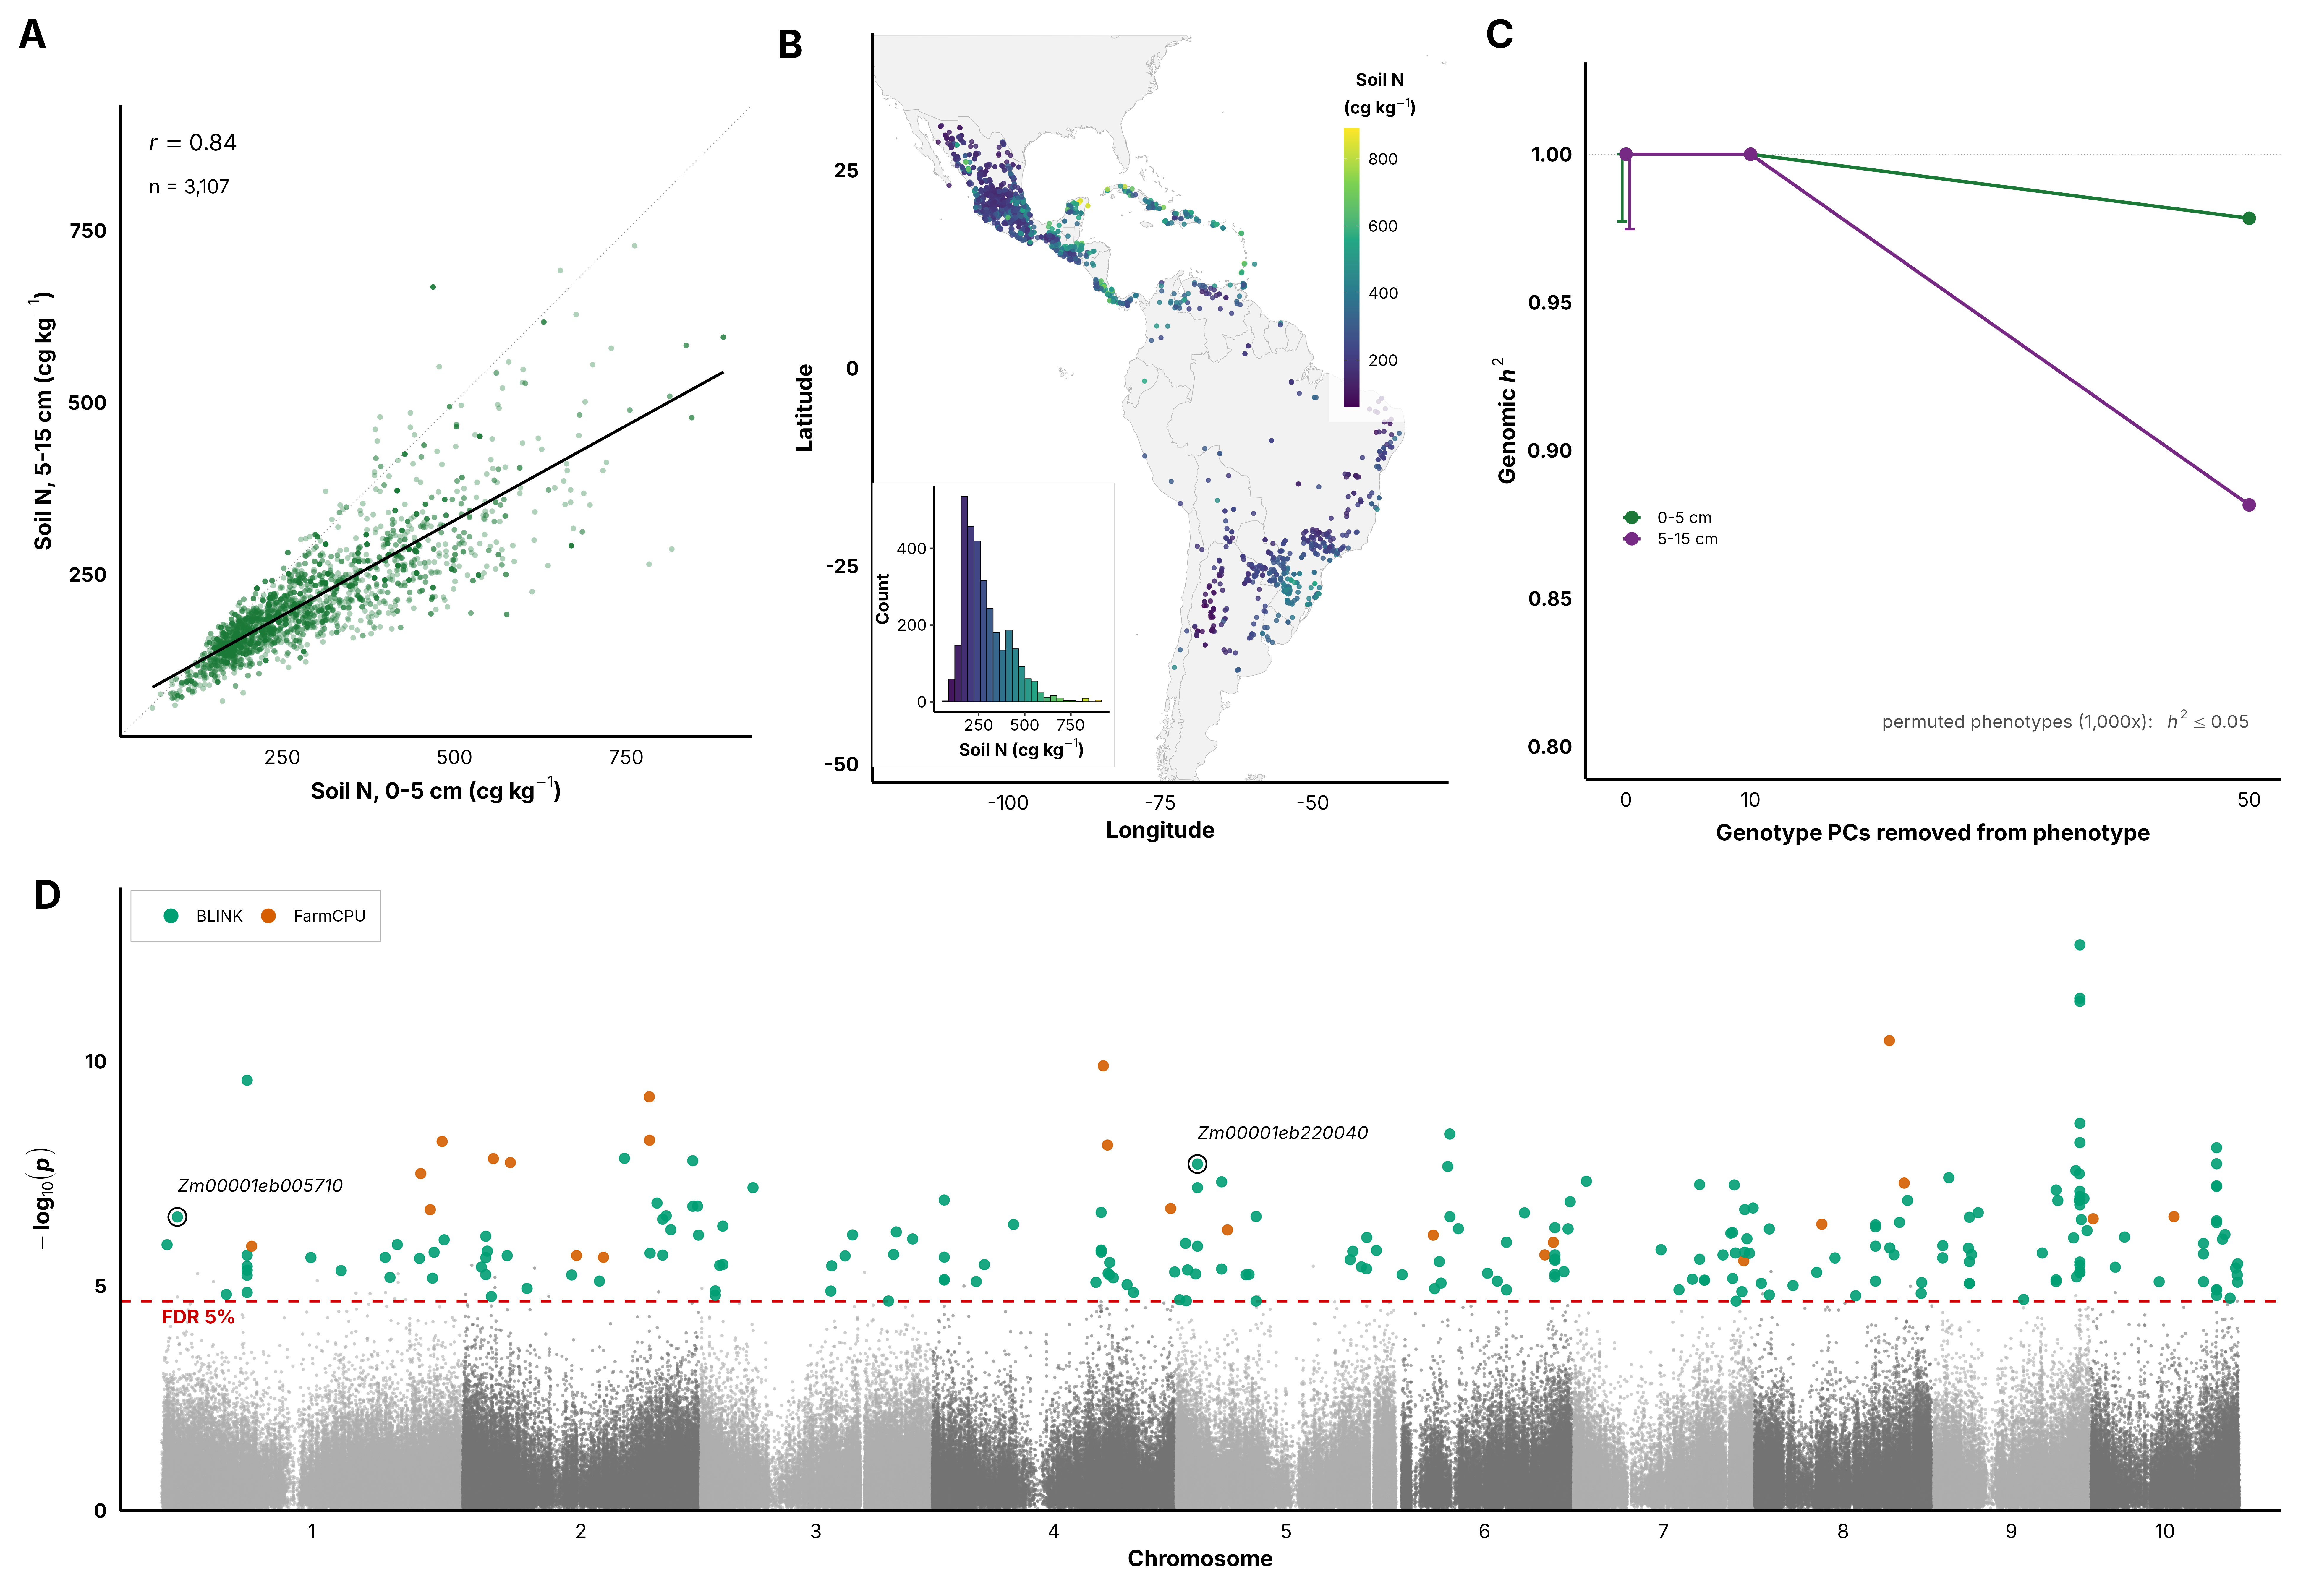
\includegraphics[width=\textwidth]{figures/Fig2_soilN.png}
  \caption{\textbf{Soil N at the collection site of 3,107 maize landraces.}
  \textbf{(A)} Soil N at 0--5\,cm vs.\ 5--15\,cm ($r = 0.84$); solid line, least-squares fit;
  dotted line, $y = x$.
  \textbf{(B)} Collection sites colored by soil N at 0--5\,cm; inset, distribution of
  soil N across accessions.
  \textbf{(C)} Genomic heritability ($h^2$) of soil N at both depths after removing
  0, 10 and 50 genotype principal components from the phenotype; error bars, 95\% CI at
  0 PCs; permuted phenotypes (1,000$\times$) gave $h^2 \leq 0.05$.
  \textbf{(D)} Manhattan plots for soil N (0--5\,cm); colored points are SNPs significant at 5\% Benjamini--Hochberg FDR in at least one model (MLM, BLINK, FarmCPU; 3 PCs), colored by the model with the lowest $P$; the SNPs near the aspartate kinase isozyme (\textit{Zm00001eb220040}) and the $\omega$-amidase (\textit{Zm00001eb005710}) are ringed and labeled. The dashed red line marks the 5\% FDR threshold. Candidate genes named in the text are labeled.}
  \label{fig:soilN_gwas}
% Alt text: TODO (required by Plant Physiology for each figure)
\end{figure*}

\subsection{Free amino acid profiles of Indian Chief and Jarvis show population-specific remodeling of the soluble amino acid pool}

To ask how the grain amino acid pool responds to yield selection, we compared Cycle~0 and Cycle~14 of Indian Chief and Jarvis, two populations in which 14 cycles of reciprocal recurrent selection shifted N allocation differently \citep{Moll1994}. We treat these profiles as evidence of changes in the grain amino acid pool, not of changes in N allocation or remobilization. Within each population, we compared total FAA, the fractions of Pro, Asn, Asp, Gln, and Glu, the N-rich FAAs (Asn + Gln + Arg + Lys + His), and FAA-derived N, correcting for these eight tests (Figure~\ref{fig:ic_j_faa}, Supplemental Table~S14).

Indian Chief changed in both total FAA and composition. Total FAA per mg increased from 1.40 in Cycle~0 to 2.46 in Cycle~14 (Wilcoxon $P = 0.0043$, BH $P = 0.017$, Figure~\ref{fig:ic_j_faa}A), with no overlap between cycles. Pro increased from 0.320 to 0.519 of total FAA (BH $P = 0.025$), whereas Asp decreased from 0.115 to 0.075 (BH $P = 0.025$) and Glu from 0.140 to 0.062 (BH $P = 0.018$), and Asn and Gln were unchanged (Figure~\ref{fig:ic_j_faa}B). In Jarvis, which had only three Cycle~0 samples, the Asp fraction increased nominally from 0.075 to 0.137 ($P = 0.019$, BH $P = 0.15$), and no other measure changed (Supplemental Table S14).

Protein-bound composition did not change in either population (Supplemental Figure~S9, Supplemental Tables~S15--S16). In Indian Chief, FAA-derived N increased from 1.75 to 2.99 per mg, but PBAA-derived N was more than 100-fold larger and unchanged, as was total amino acid-derived N ($P = 0.42$, Supplemental Figure~S10, Supplemental Table~S17). Thus, after 14 cycles of selection, Indian Chief had more free amino acids and a composition shifted from Asp and Glu toward Pro, whereas Jarvis showed no corrected change, and neither population changed in the protein-bound pool that holds most grain amino acid N.

\begin{figure*}[ht!]
\centering
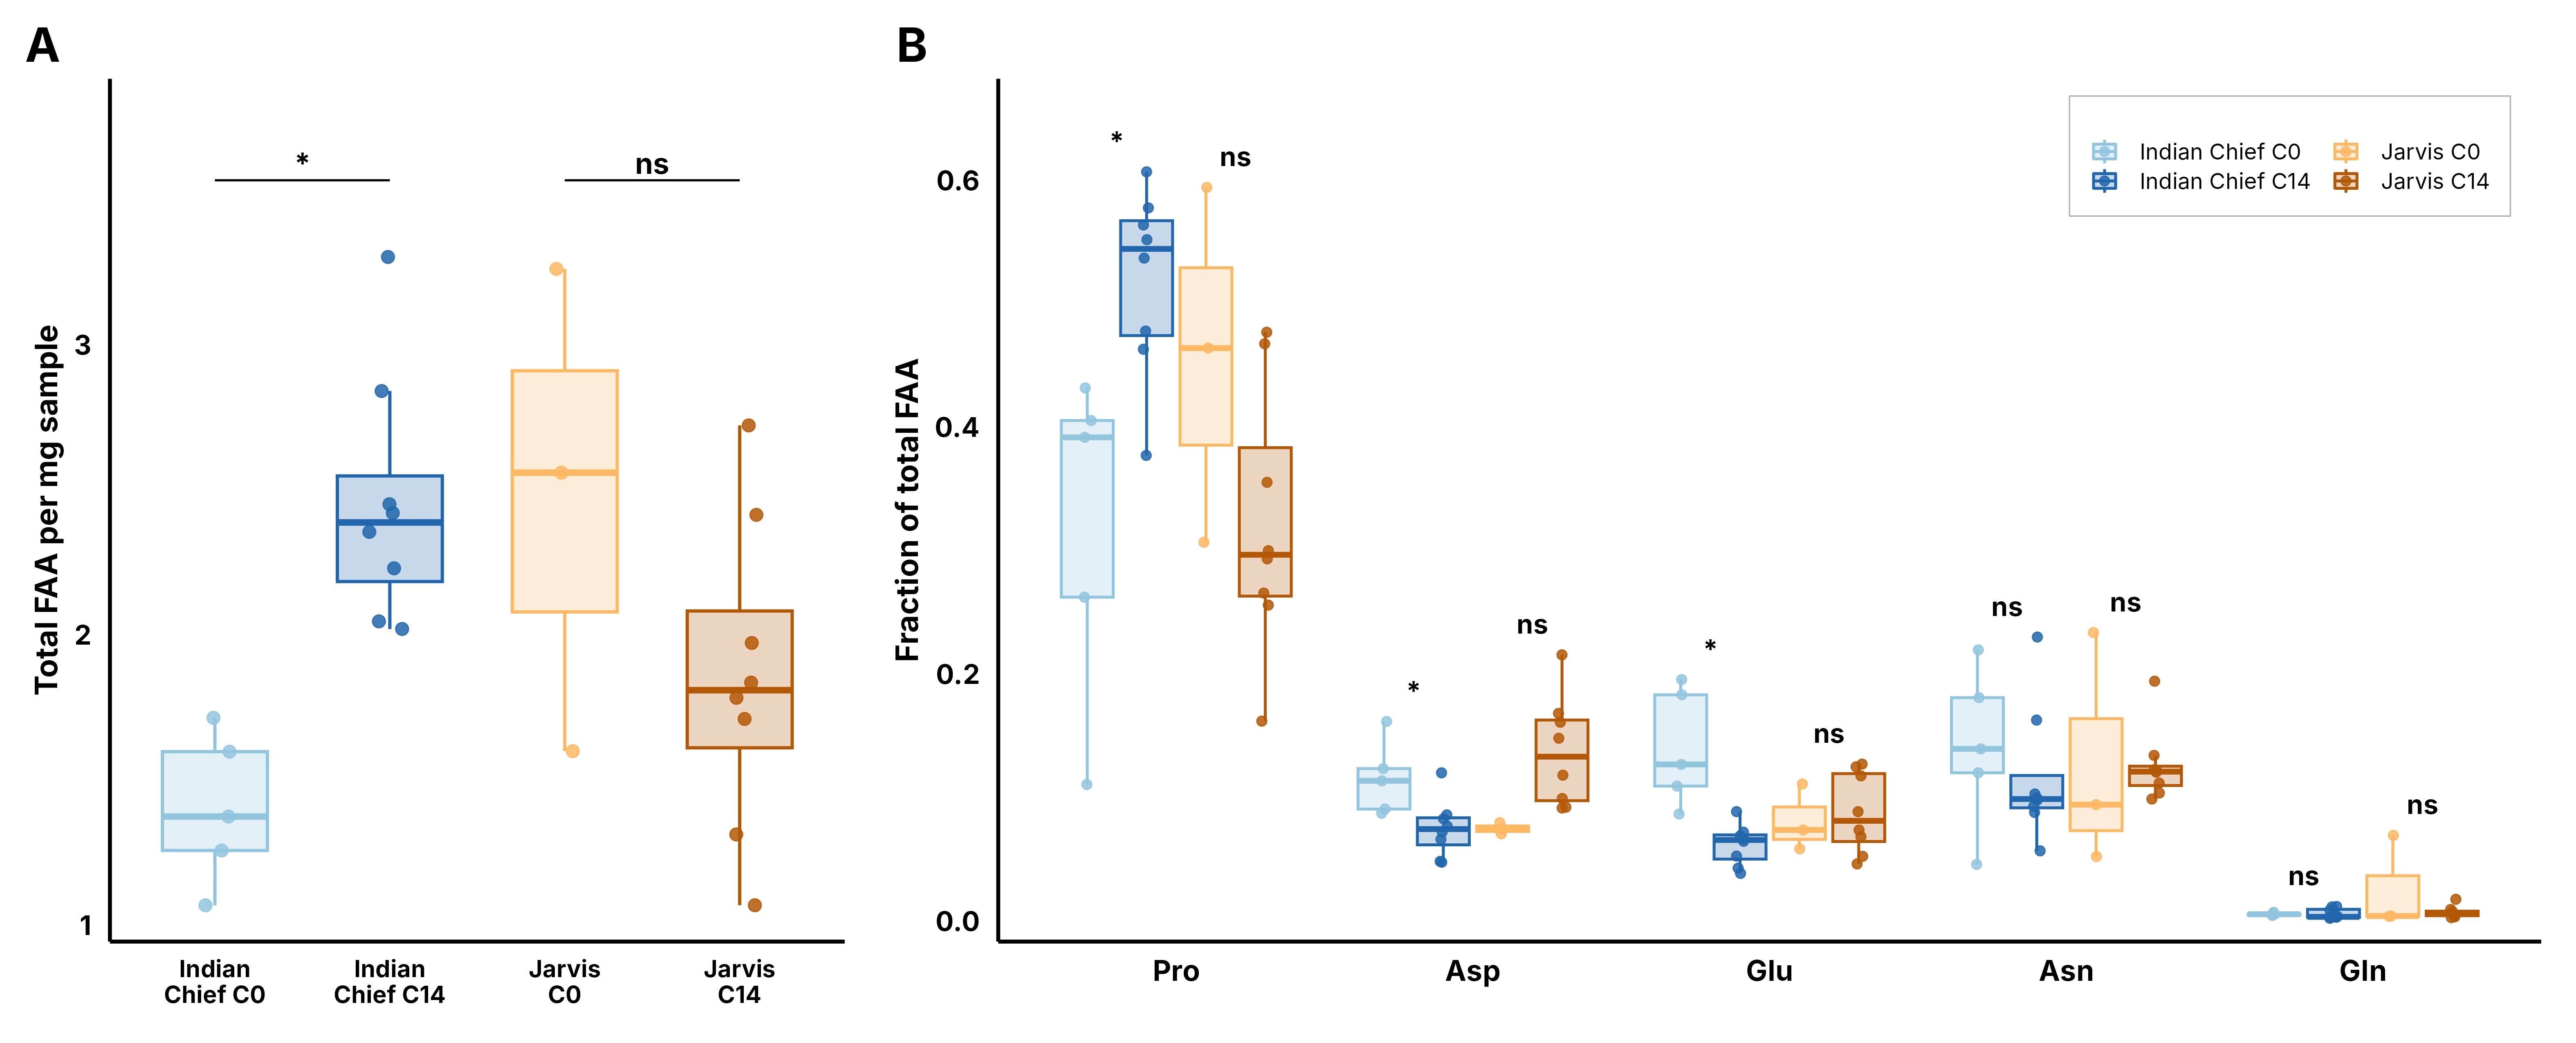
\includegraphics[width=\textwidth]{figures/Fig3_IC_J_FAA.png}
\caption{
\textbf{Free amino acid (FAA) pool and composition in Indian Chief and Jarvis before (C0) and after (C14) 14 cycles of reciprocal recurrent selection.} \textbf{(A)} Total FAA per mg sample. \textbf{(B)} Fractions of total FAA for Pro, Asp, Glu, Asn and Gln. Points are biological samples, each the mean of three technical replicates; boxes show the median and interquartile range. Within each population, C0 and C14 were compared with two-sided Wilcoxon rank-sum tests, and $P$ values were adjusted with the BH method; * adjusted $P < 0.05$; ns, not significant.
}
\label{fig:ic_j_faa}
% Alt text: TODO (required by Plant Physiology for each figure)
\end{figure*}

\subsection{Skim sequencing reveals that Indian Chief and Jarvis diverged during reciprocal recurrent selection}

We skim sequenced 379 individuals from Indian Chief and Jarvis at Cycle~0 and Cycle~14 (mean depth 0.73$\times$, Supplemental Figure~S11). Because depth was higher at Cycle~14 than at Cycle~0, hard-called genotypes would differ between cycles for technical reasons, so we used genotype likelihoods throughout (Supplemental Figure~S12). Ancestry estimation separated the four population--cycle groups, with runs converging at $K = 4$, where each group formed a distinct cluster (Figure~\ref{fig:ic_j_structure}A). At $K = 2$--3, Indian Chief Cycle~0 was inferred as a mixture of the Jarvis Cycle~0 and Indian Chief Cycle~14 clusters. In the PCA, PC1 (14.3\%) separated Indian Chief Cycle~14 from Jarvis Cycle~14, with both Cycle~0 groups near the center, and PC2 (6.7\%) separated Cycle~14 from Cycle~0 (Figure~\ref{fig:ic_j_structure}B).

$F_{ST}$ between Indian Chief and Jarvis nearly doubled, from 0.111 at Cycle~0 to 0.211 at Cycle~14, on all ten chromosomes (Figure~\ref{fig:ic_j_structure}C). Because Cycle~14 was sequenced more deeply, which should reduce rather than inflate $F_{ST}$, the increase is unlikely to be a depth artifact. This divergence is expected under reciprocal recurrent selection, which favors complementary alleles \citep{Comstock1949RRS}, and is reinforced by drift in small, separately maintained populations.

%===================== FIGURE 4 =====================
\begin{figure*}[ht!]
    \centering
    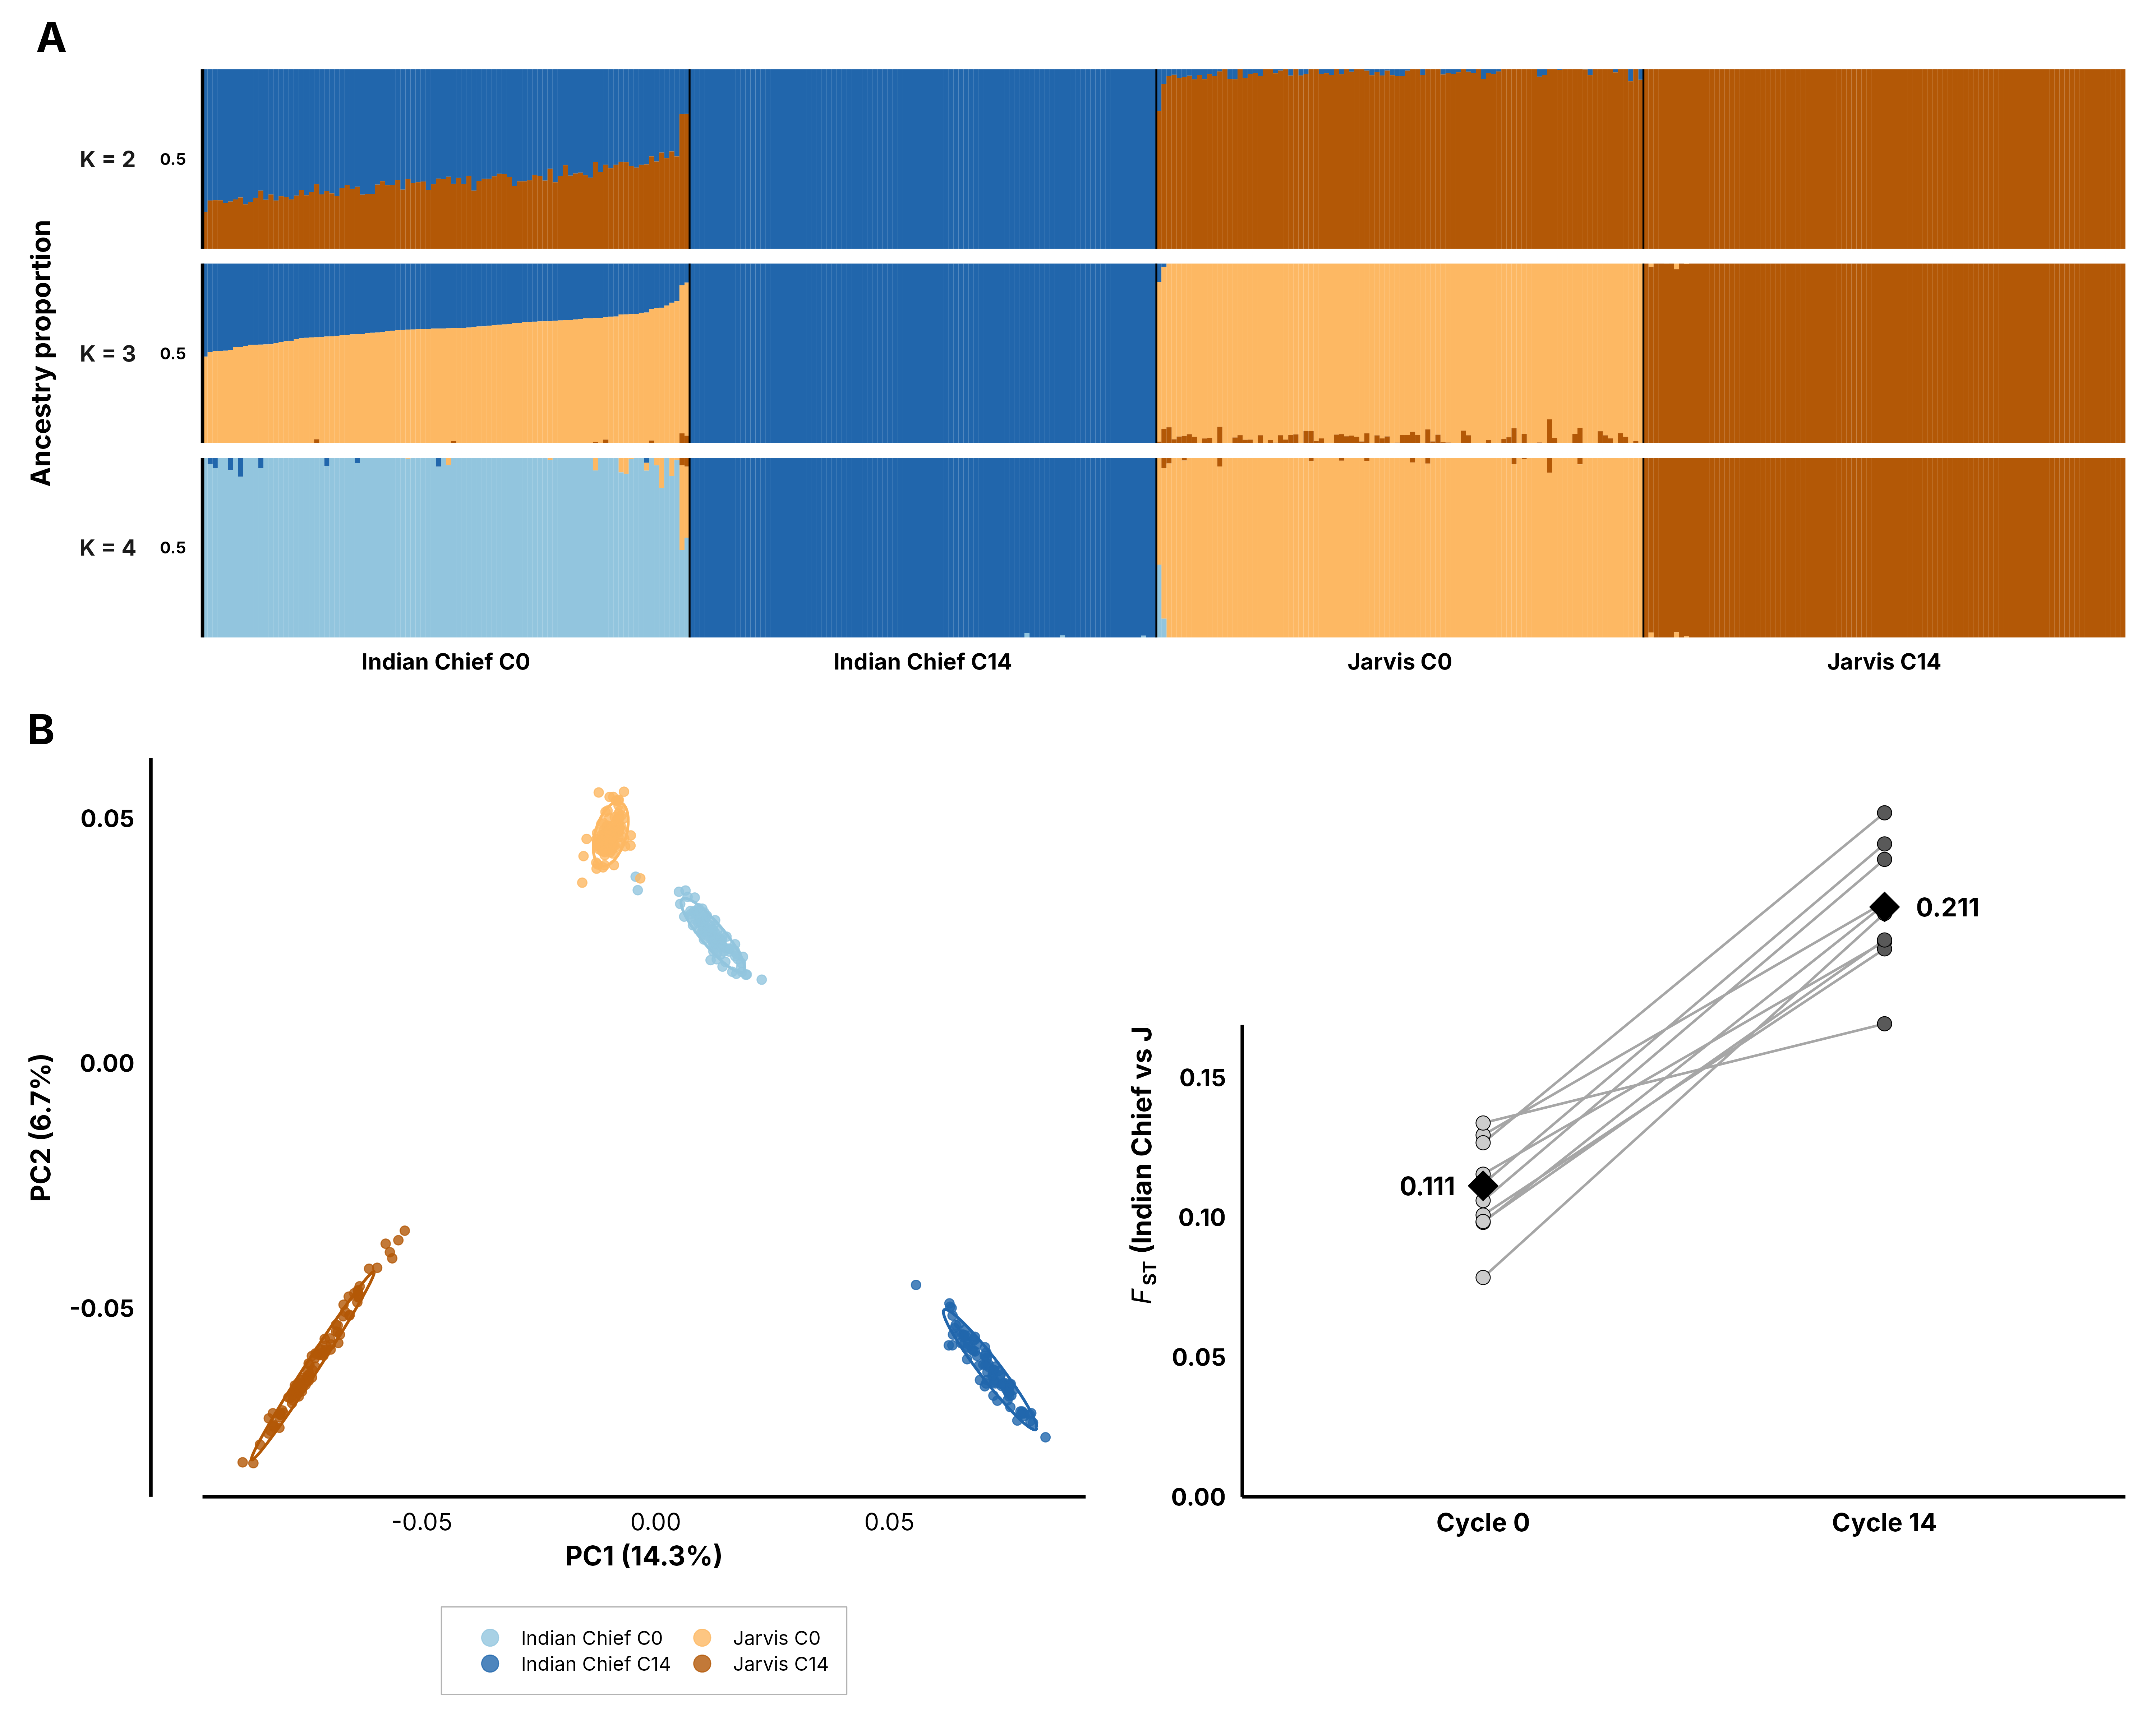
\includegraphics[width=\textwidth]{figures/Fig4_IC_J_structure.png}
    \caption{\textbf{Indian Chief and Jarvis divergence during 14 cycles of reciprocal recurrent selection.} All panels use genotype likelihoods. \textbf{(A)} Unsupervised ancestry proportions for $K = 2$--4 (thinned to one per 10~kb); each bar is one individual, and each cluster is colored by the group with the highest mean membership. $K = 4$ is the largest $K$ at which independent runs converged. \textbf{(B)} Principal component analysis of the genotype-likelihood covariance matrix; ellipses enclose 90\% of each group. Individuals with lower depth carry less information and lie closer to the center of their group. \textbf{(C)} $F_{ST}$ between Indian Chief and Jarvis at Cycle 0 and Cycle 14, estimated from the joint site-frequency spectrum of each pair; gray lines connect the same chromosome and black diamonds give the genome-wide value.}
    \label{fig:ic_j_structure}
% Alt text: TODO (required by Plant Physiology for each figure)
\end{figure*}

\subsection{$F_{ST}$ scans identify population-specific candidate regions in Indian Chief and Jarvis}

Before scanning for regions of high differentiation, we asked how much allele-frequency change drift could explain. Each cycle was formed from the selfed progenies of the 20 best plants per population \citep{MollStuber1971}, implying an effective population size ($N_e$) of at most 20. Genome-wide mean $F_{ST}$ between Cycle~0 and Cycle~14 was 0.095 in Indian Chief and 0.114 in Jarvis (Figure~\ref{fig:ic_j_fst}), values reproduced by neutral simulations at $N_e \approx 30$ and 26 (Supplemental Figure~S13). Most genome-wide change is therefore consistent with drift, as found for other maize populations under reciprocal recurrent selection \citep{Gerke2015DriftRRS}, and at this $N_e$ individual outlier regions cannot be formally distinguished from drift. We therefore treat the scans as exploratory.

We retained the top 5\% of $F_{ST}$ windows in each population (109 of 2,162 in Indian Chief and 108 of 2,151 in Jarvis), which contained 2,001 and 1,179 genes (Figure~\ref{fig:ic_j_fst}, Supplemental Tables~S18--S21). Only five regions (2.5~Mb, 73 genes) were in the top 5\% in both populations, no more than expected by chance ($P = 0.80$), and the amino acid GWAS loci fell in top windows no more often than expected (8.9\% of loci and of the genome, $P = 0.52$).

Because each candidate set contains more than 1,000 genes, we focused on genes in the functions highlighted by the GWAS (Asp-family and Glu/Gln metabolism, amino acid and N transport, and protein turnover) and treat them as candidates of interest rather than evidence of selection. Indian Chief regions included aspartate-semialdehyde dehydrogenase (\textit{Zm00001eb214360}), threonine synthase (\textit{Zm00001eb294790}), two glutamate dehydrogenases (\textit{Zm00001eb060520}, \textit{Zm00001eb162300}), a glutamine synthetase (\textit{Zm00001eb162900}), the glutamine amidotransferase also associated with free Pro in the GWAS (\textit{Zm00001eb217220}), the senescence protease \textit{SAG39} (\textit{Zm00001eb214780}), and autophagy-related genes. Jarvis regions included aspartate kinase (\textit{Zm00001eb094670}), an aspartate aminotransferase (\textit{Zm00001eb152450}, GOT1/THP3), LHT-like (\textit{Zm00001eb132750}) and ProT-like (\textit{Zm00001eb159580}) transporters, NPL4-like protein 1 (\textit{Zm00001eb146560}), and two CC-type glutaredoxins (\textit{Zm00001eb131830}, \textit{Zm00001eb131840}). These candidates require functional validation.

%===================== FIGURE 5 =====================
\begin{figure*}[ht!]
    \centering
    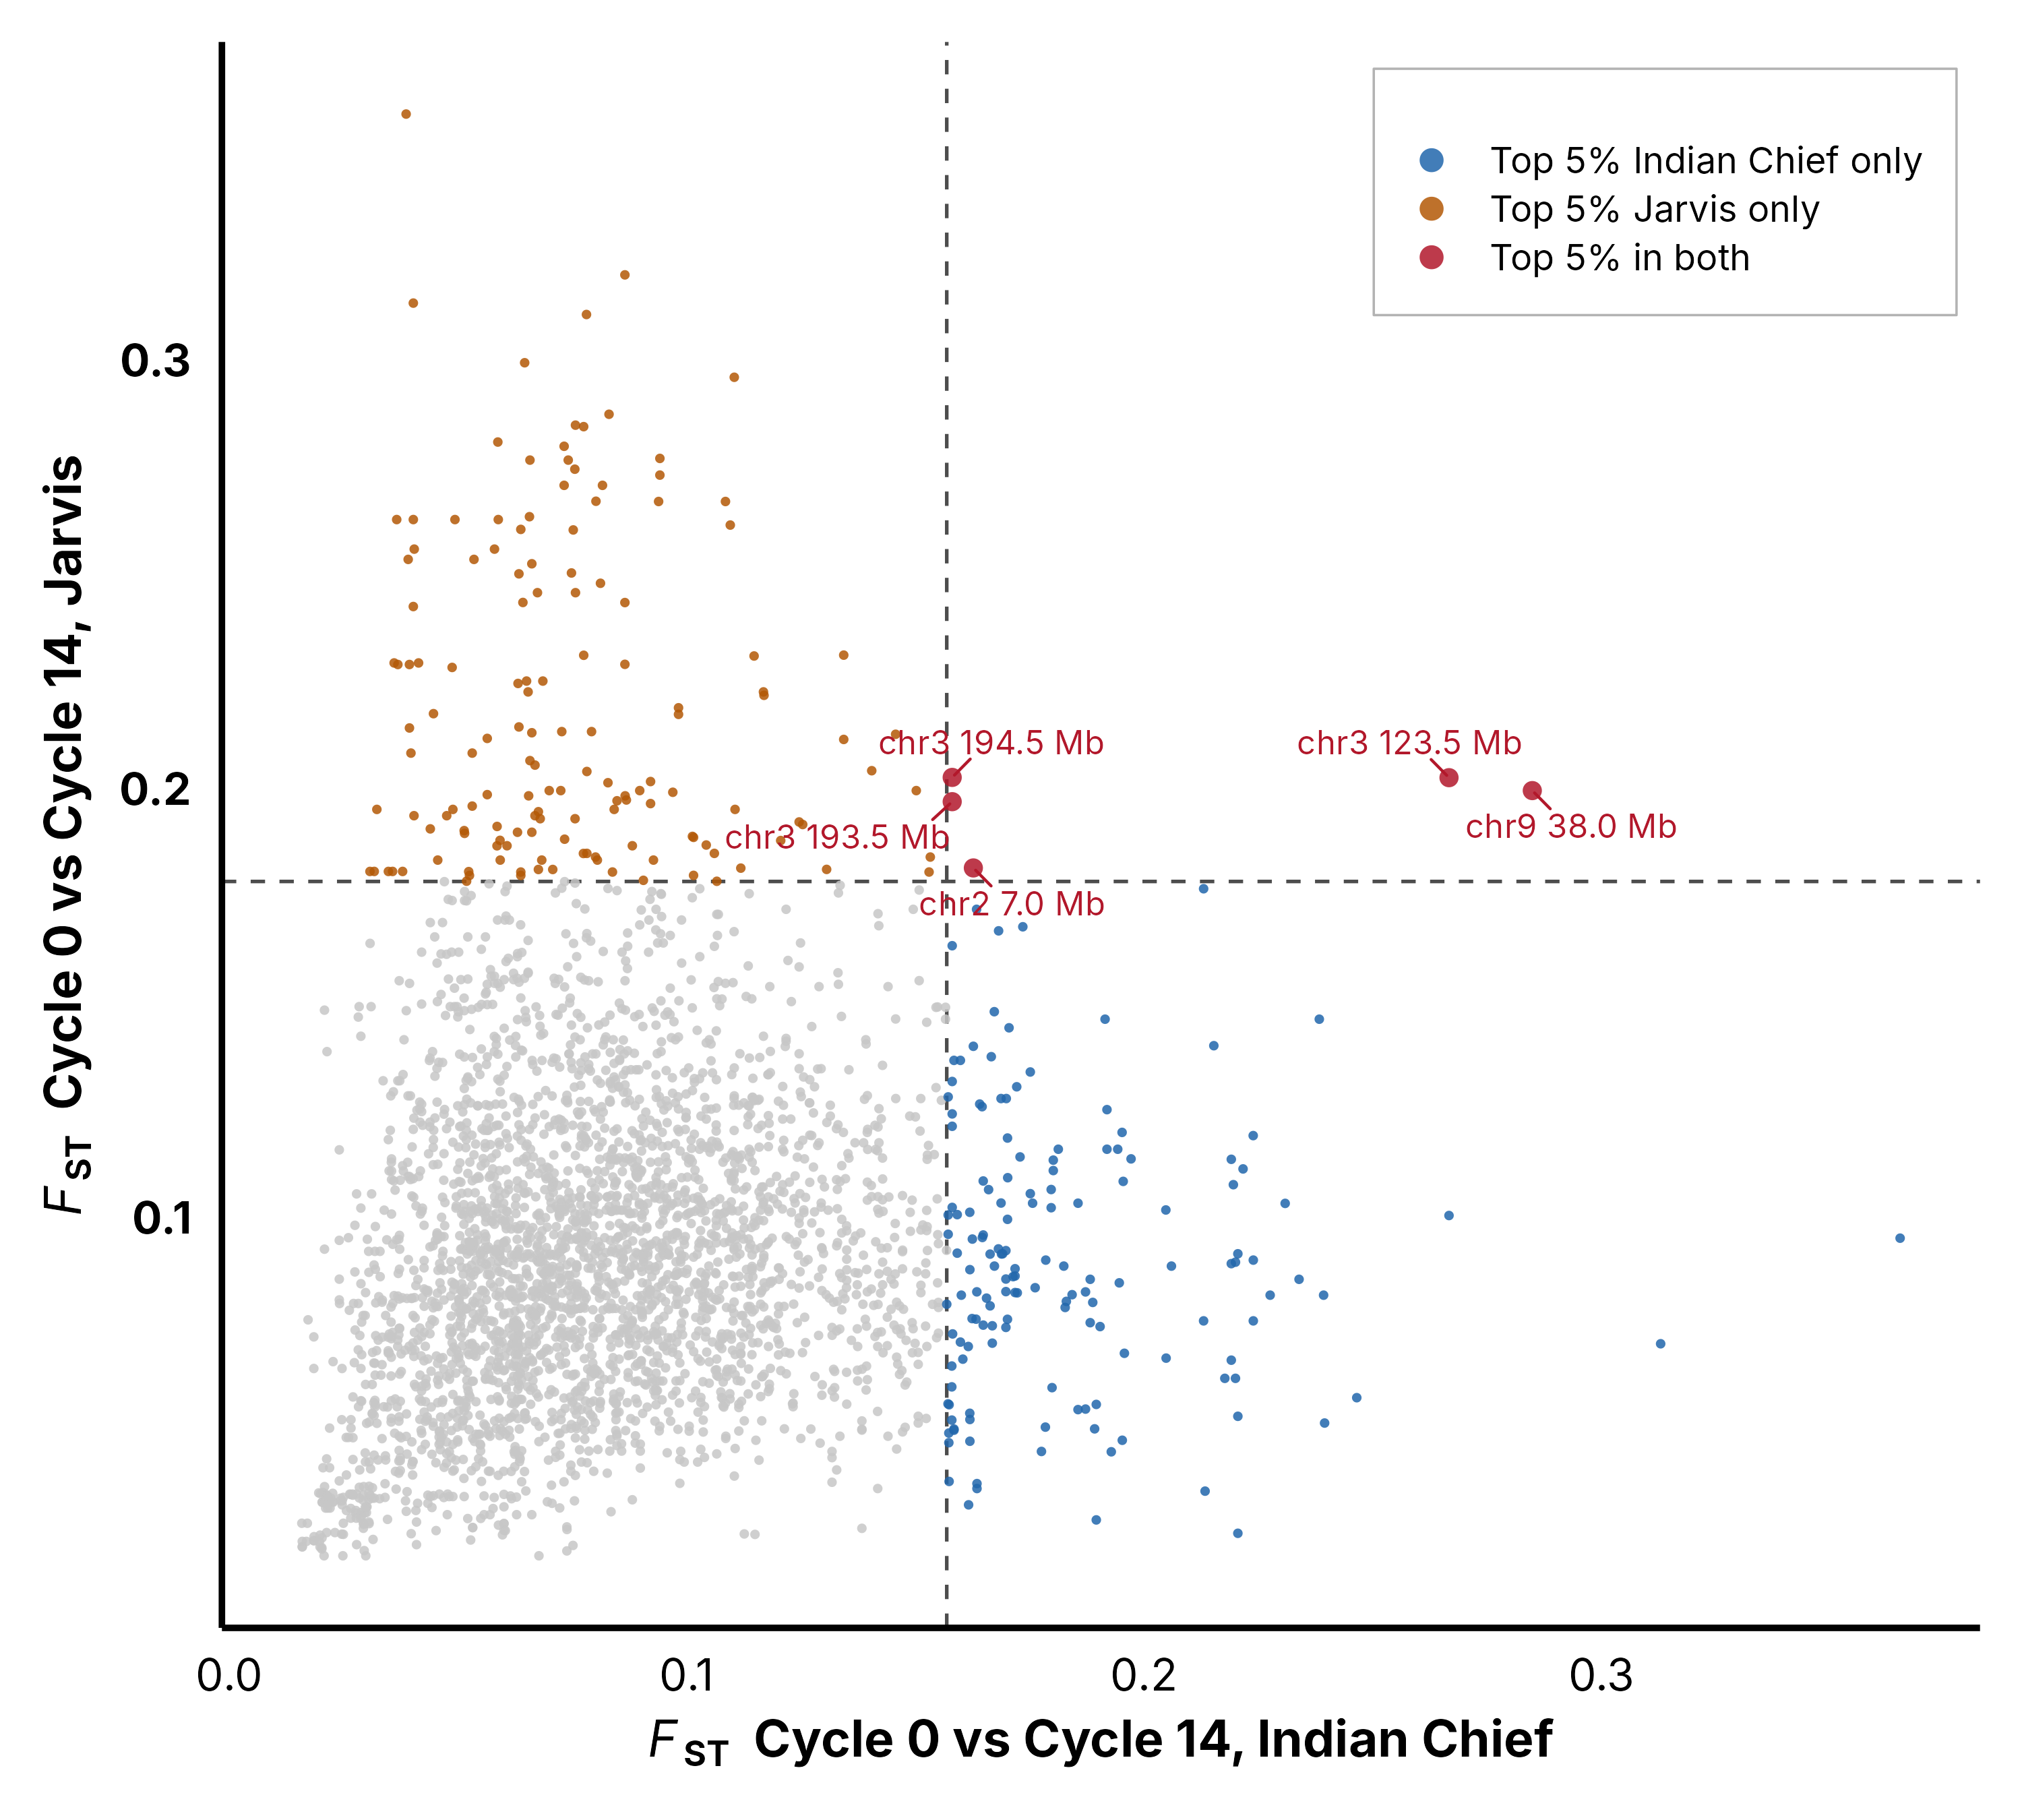
\includegraphics[width=0.75\textwidth]{figures/Fig5_IC_J_Fst_scan.png}
    \caption{\textbf{Candidate regions of differentiation between Cycle 0 and Cycle 14} $F_{ST}$ between Cycle 0 and Cycle 14 in Indian Chief ($x$-axis) and Jarvis ($y$-axis), estimated from genotype likelihoods and summarized in spline-defined windows. Each point is a genomic segment bounded by the window boundaries of either population, and carries the $F_{ST}$ of the Indian Chief and Jarvis windows that contain it. Dashed lines mark the top 5\% of windows in each population ($F_{ST} \geq 0.157$ in Indian Chief and $\geq 0.178$ in Jarvis). Blue and orange, top 5\% in one population only; red, top 5\% in both, labeled with chromosome and position.}
    \label{fig:ic_j_fst}
% Alt text: TODO (required by Plant Physiology for each figure)
\end{figure*}

\subsection{The aspartate-to-homoserine pathway recurs across the three populations}

To test whether the three populations implicate the same metabolic pathways, we asked whether any of 468 CornCyc pathways \citep{Hawkins2021PMN} contained candidate genes from more of the four analyses than expected by chance. We used strict candidate sets (Bonferroni-significant GWAS SNPs and the top 3\% of $F_{ST}$ windows), because larger sets add background genes that hit many pathways by chance. L-homoserine biosynthesis had candidates from all four analyses, had the lowest permutation-based empirical $P$ ($P = 0.00034$), and was the only pathway that remained significant after correction (corrected $P = 0.021$, Figure~\ref{fig:pathway_recurrence}). Each analysis implicated a different enzyme, homoserine dehydrogenase (\textit{Zm00001eb405410}) in the amino acid GWAS, an aspartate kinase isozyme (\textit{Zm00001eb220040}) in the soil N GWAS, aspartate-semialdehyde dehydrogenase (\textit{Zm00001eb214360}) in Indian Chief, and aspartate kinase (\textit{Zm00001eb094670}) in Jarvis. L-lysine biosynthesis VI also had candidates from all four analyses ($P = 0.0030$), because it shares the aspartate kinase and aspartate-semialdehyde dehydrogenase steps.

Across 12 combinations of GWAS and $F_{ST}$ thresholds (Supplemental Figure~S14), the same four genes were recovered with the top 5\% or 3\% of windows, and L-homoserine biosynthesis ranked first five times and second three times. Lower ranks occurred only with the top 1\% of windows, and with the largest candidate sets the pathway was not significant after correction (corrected $P = 0.68$). Thus, the pathway ranked consistently across thresholds, while corrected significance depended on candidate-set size.

\begin{figure*}[ht!]
  \centering
  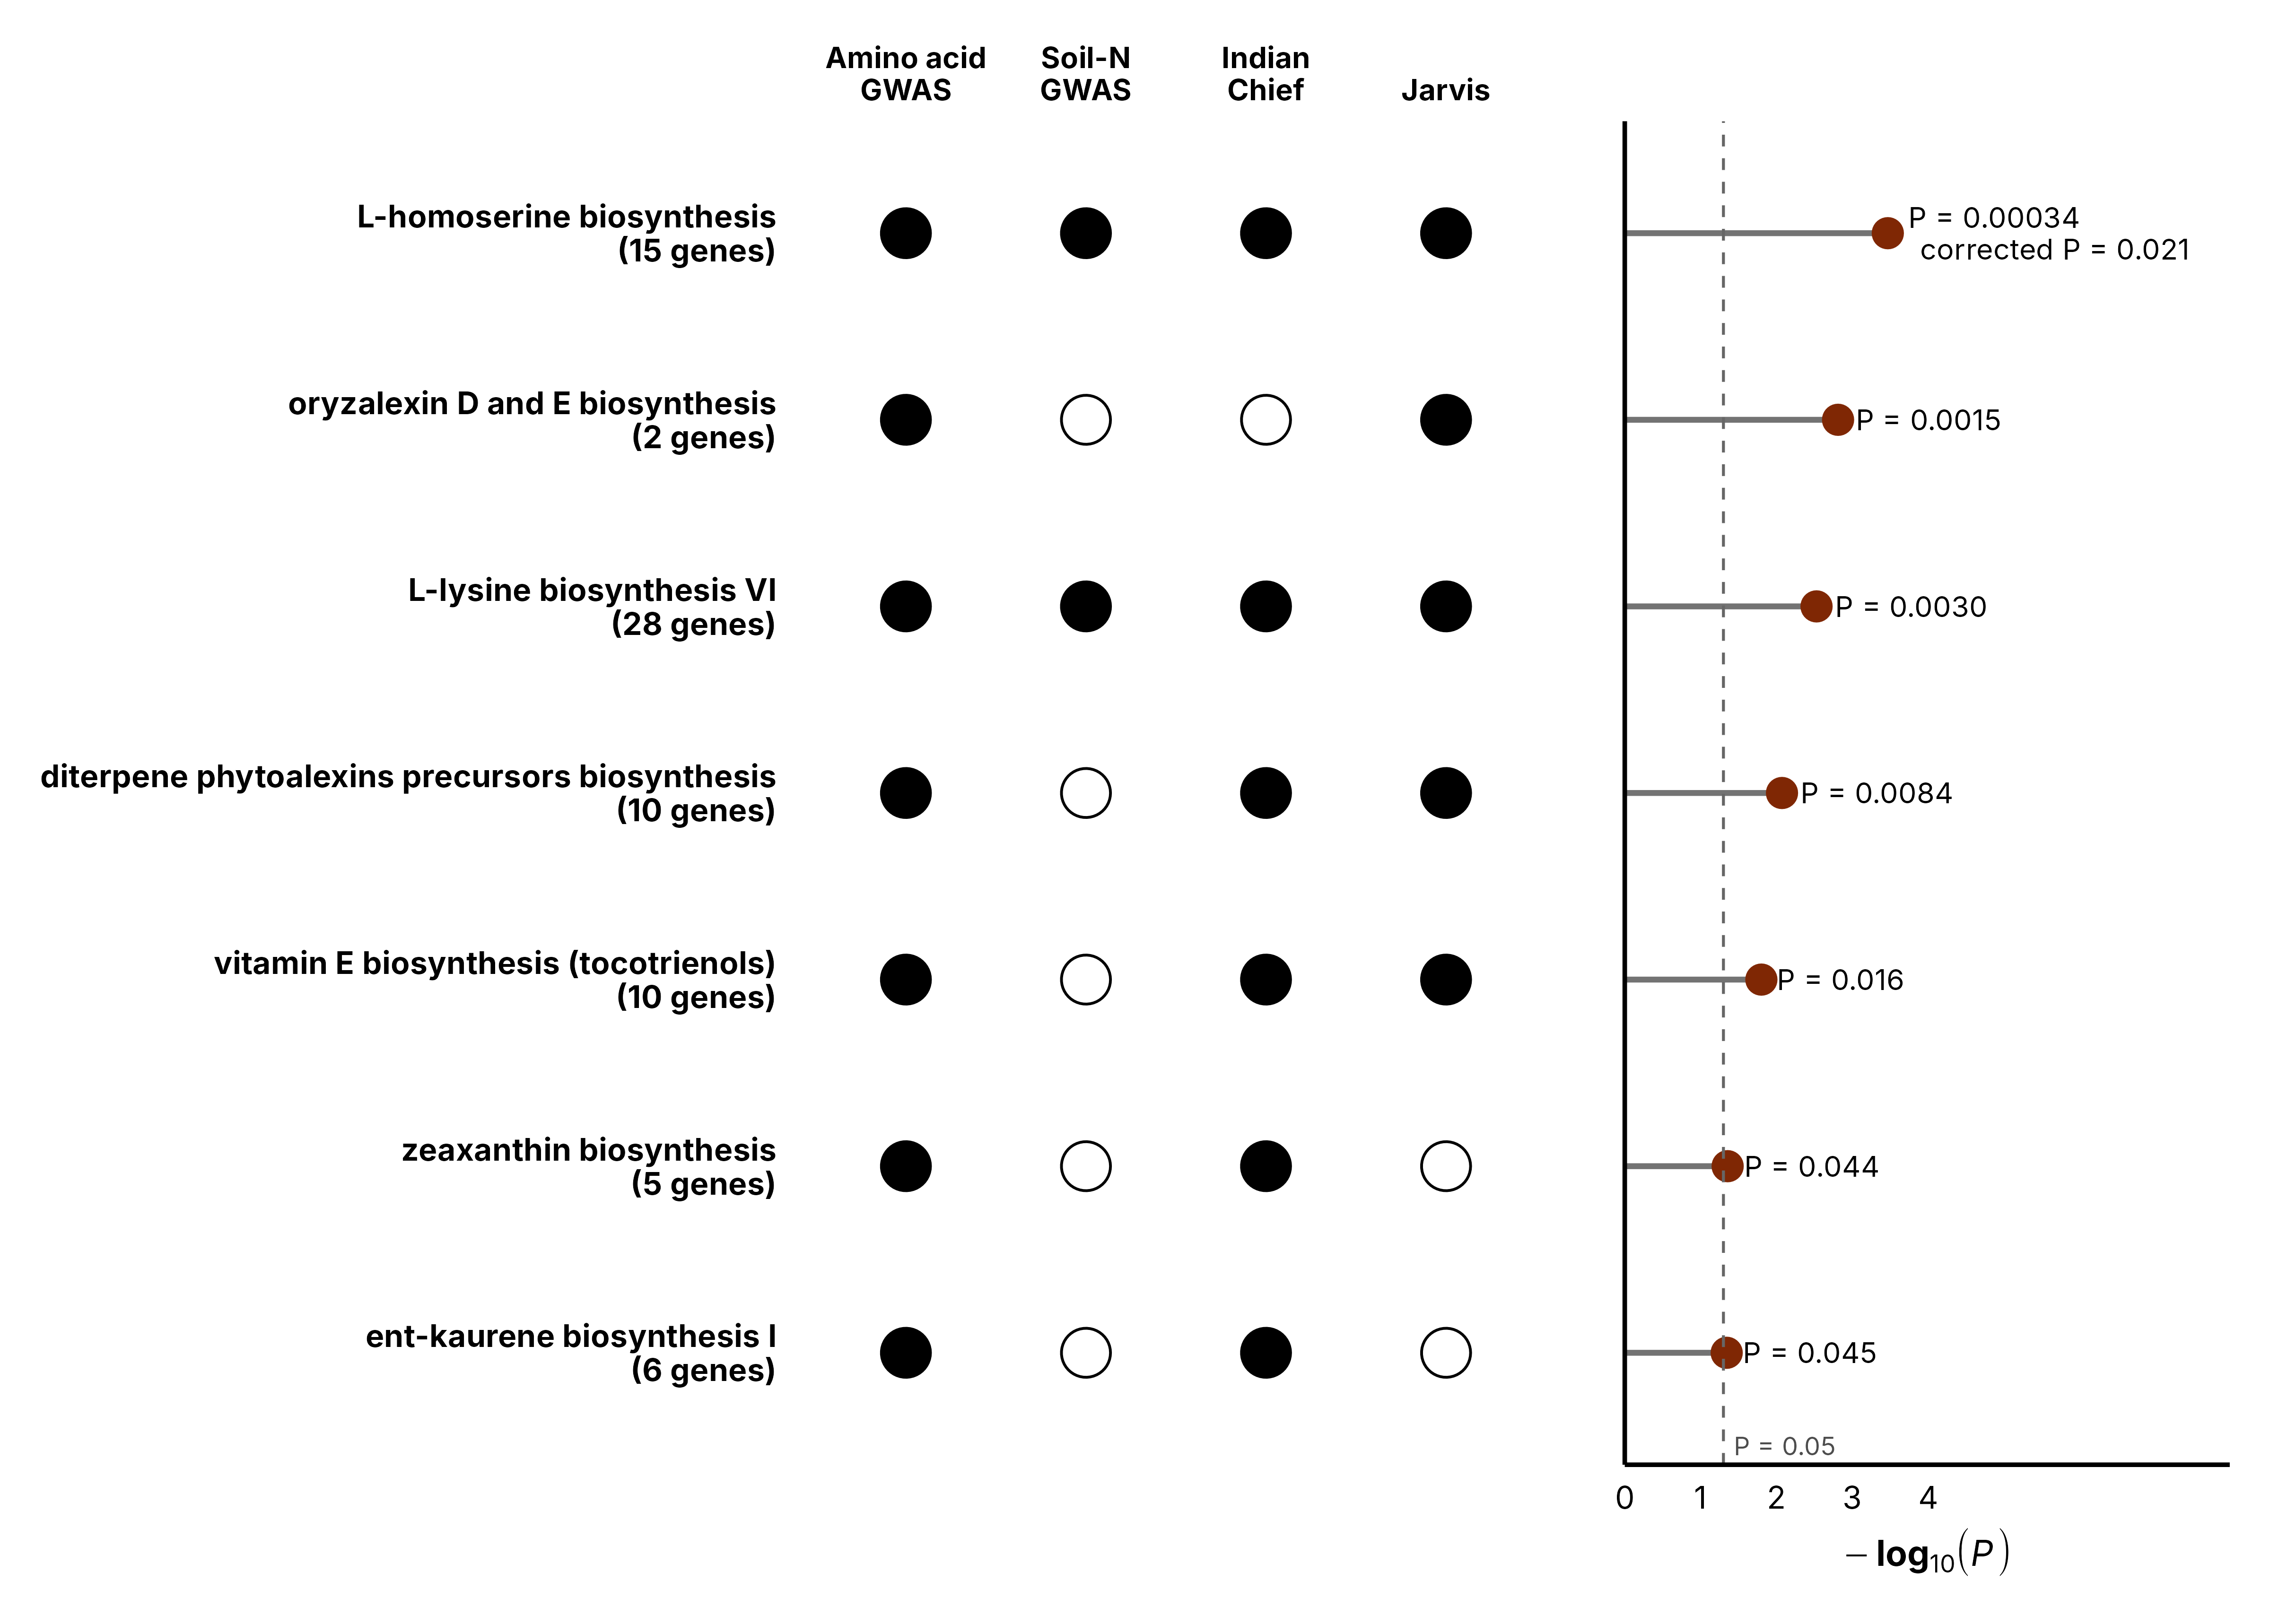
\includegraphics[width=\textwidth]{figures/Fig_pathway_recurrence.png}
    \caption{\textbf{The L-homoserine biosynthesis pathway recurs across all four analyses.} All CornCyc pathways with uncorrected permutation $P < 0.05$ for recurrence across the amino acid GWAS, soil-N GWAS and the Indian Chief and Jarvis $F_{ST}$ scans, using Bonferroni-significant GWAS SNPs and the top 3\% of $F_{ST}$ windows. Left, filled circles mark analyses with at least one candidate gene in the pathway; numbers in brackets give the number of maize genes in the pathway. Right, pathway-specific permutation-based empirical $P$ for the observed number of analyses hitting the pathway; dashed line, $P = 0.05$. The corrected $P$ (minimum-$P$ correction across all 468 pathways) is shown for the only pathway that remained significant.}
  \label{fig:pathway_recurrence}
% Alt text: TODO (required by Plant Physiology for each figure)
\end{figure*}

\section{Discussion}

We tested whether natural variation in grain amino acids, genetic variation linked to soil N, and yield selection implicate the same N-metabolism functions in maize. Although most candidates were analysis-specific, each analysis implicated a different enzyme in the aspartate-to-homoserine pathway, the only pathway that remained significant after correction. Candidates in each population also pointed to the aspartate--glutamate junction and to amino acid transport and protein turnover, in ways consistent with each population's phenotype. These annotation-based candidates require functional validation.

\subsection{Loci shared by many amino acid traits point to protein turnover and membrane protein biogenesis rather than specific biosynthetic steps}

Few GWAS loci were shared across many amino acid phenotypes. The most interpretable case is the chromosome 4 locus at 174.57 Mb, associated with eight phenotypes (including Ala, Val, Lys, Phe, and Thr) spanning four biosynthetic families, and adjacent to \textit{Zm00001eb190800}, encoding a peptidase A1 (pepsin-like aspartic protease) (Figure~\ref{fig:amino_locus_manhattan}). Aspartic proteases are known to drive bulk protein turnover. In senescing tobacco, chloroplast CND41 degrades Rubisco, and reduced CND41 increases Rubisco retention under N limitation \citep{Kato2004CND41}. Rubisco breakdown is a major source of amino acids released during senescence \citep{Feller2008Rubiscolytics}, although A1 proteases also act in development and stress responses \citep{Soares2019AtypicalAP}. A single locus affecting amino acids from four biosynthetic families is more easily explained by a change in protein degradation than by a change in one biosynthetic enzyme, which makes \textit{Zm00001eb190800} a plausible candidate for functional testing.

The chromosome 9 locus implicates the endomembrane system. A $\sim$13 kb region associated with nine phenotypes (including total free amino acids) spans \textit{Zm00001eb394360} and \textit{Zm00001eb394380}. \textit{Zm00001eb394360} encodes ER membrane protein complex subunit 4, which inserts transmembrane proteins into the ER \citep{Guna2018EMC}, and \textit{Zm00001eb394380} encodes rhomboid-like protein 19, an intramembrane serine protease annotated for Golgi-to-ER retrograde transport. Although the functions of most plant rhomboid-like proteins remain unknown \citep{Lavell2021RBL10}, both genes act in the ER--Golgi system that processes transporters and secreted proteins involved in amino acid and N movement \citep{Brandizzi2018ERGolgi}, so either could affect the overall free amino acid pool. Because the associations do not clearly separate these genes from nearby genes (including a DUF2404 membrane protein at the chromosome 4 locus), both loci should be treated as positional candidates, and kernel expression and mutant analyses are the most direct tests.

\subsection{The aspartate-to-homoserine pathway links soil-N adaptation, recurrent selection, and grain amino acid variation}

Asn was the most abundant free amino acid in the Goodman--Buckler panel and, because of its high N-to-C ratio, is a major N transport and storage form in plants \citep{Lea2007Asparagine}. It is synthesized from Asp by asparagine synthetase using the amide N of Gln, and catabolism returns carbon to Asp or oxaloacetate \citep{Lea2007Asparagine}. Asp is thus both the precursor of Asn and the entry point to the Asp-family pathway that produces Lys, Thr, Met, and Ile \citep{Han2021Aspartate, Wang2018AspSeeds, Viola2001AspartatePathway}. Pathway flux is regulated mainly by feedback inhibition of aspartate kinase by Lys and Thr, and of dihydrodipicolinate synthase by Lys \citep{Azevedo2006AspPathway, Jander2009AspArabidopsis}. This pathway was implicated by all four analyses. L-homoserine biosynthesis had a candidate gene in every analysis, had the lowest permutation-based empirical $P$ of the 468 CornCyc pathways, and was the only pathway that remained significant after correction (Figure~\ref{fig:pathway_recurrence}).

Across analyses, implicated genes spanned the Asp to homoserine pathway. Jarvis regions included aspartate kinase (\textit{Zm00001eb094670}), the first committed step \citep{Viola2001AspartatePathway}, and \textit{ask2} expression is linked to Met accumulation in developing kernels \citep{Duo2026Ask2}. The only soil N SNP significant in all three GWAS models, which also passed both tests for confounding with geography and climate, was near another aspartate kinase (\textit{Zm00001eb220040}). Indian Chief regions included aspartate-semialdehyde dehydrogenase (\textit{Zm00001eb214360}), and the amino acid GWAS implicated homoserine dehydrogenase (\textit{Zm00001eb405410}), the first committed step to Thr and Met. Further downstream, Indian Chief regions included threonine synthase (\textit{Zm00001eb294790}) and methionine synthase (\textit{Zm00001eb052750}), the latter also near a soil-N SNP.

Together, three populations with different germplasm and study designs point to the same short pathway, with each analysis implicating a different enzyme, and L-homoserine biosynthesis ranked first or second among 468 pathways across candidate thresholds (Supplemental Figure~S14). Drift could still contribute to the $F_{ST}$ candidate regions given $N_e \approx 25$--30 (Supplemental Figure~S13), and the soil-N alleles, although they came from many independent collection sites (Supplemental Figure~S8), may partly reflect shared ancestry. These genes are therefore strong candidates for direct tests, such as comparing Asp-family amino acids among lines with alternative alleles at \textit{Zm00001eb405410}, \textit{Zm00001eb220040}, \textit{Zm00001eb214360}, and \textit{Zm00001eb094670}. Because Asp is the precursor of Asn and exchanges amino groups with Glu, variation at the entry to the Asp-family pathway could shift how Asp-derived N is allocated among Asn, Asp-family amino acids, and the Glu/Gln pool. Links from Asp to Glu/Gln and the $\omega$-amidase pathway are discussed next.

\subsection{Candidate genes at the aspartate--glutamate junction link amino acid N with C--N recycling}

Glutamate exchanges amino groups with the TCA-cycle intermediate 2-oxoglutarate, which provides the carbon skeleton for ammonium assimilation through the GS/GOGAT cycle and glutamate dehydrogenase, and whose level signals C and N status in many organisms \citep{Huergo2015TwoOG}. Together, Asp, Asn, Glu, and Gln make up most of the free amino acid pool and are major N transport forms in plants \citep{McAllister2016AAT}. Because no Glu/Gln pathway recurred across analyses, we discuss these junction candidates individually.

Each analysis implicated different genes at the junction. On the Asp side, Jarvis regions contained the aspartate aminotransferase \textit{Zm00001eb152450} (GOT1), which interconverts Asp and 2-oxoglutarate with oxaloacetate and Glu \citep{Han2021Aspartate, Zhou2009AspAT}. This gene was recently identified as \textit{THP3}, whose teosinte alleles improve N assimilation and seed protein in maize \citep{Huang2026THP3}. In contrast, overexpressing a cytosolic aspartate aminotransferase from alfalfa in \textit{Brassica napus} did not increase N use efficiency \citep{McAllister2016AAT}, suggesting that the effects of this enzyme depend on the isoform and the tissue in which it is expressed. The soil-N GWAS identified an $\omega$-amidase (\textit{Zm00001eb005710}) that completes Asn/Gln transaminase routes by returning carbon to oxaloacetate and 2-oxoglutarate while releasing ammonia \citep{Zhang2014OmegaAmidase}.

On the Glu side, the clearest case is Indian Chief, the only population whose free amino acid profile changed (Figure~\ref{fig:ic_j_faa}). Most of the Cycle 14 increase in total free amino acids was Pro, so the lower Asp and Glu fractions largely reflect Pro accumulation. Indian Chief regions included two glutamate dehydrogenases (\textit{Zm00001eb060520}, \textit{Zm00001eb162300}), a glutamine synthetase (\textit{Zm00001eb162900}), and a class I glutamine amidotransferase (\textit{Zm00001eb217220}) that was also a candidate for free Pro in the amino acid GWAS, but no genes for Pro synthesis. GDH mutants show altered amino acid profiles under carbon limitation \citep{Miyashita2008GDH, Dellero2020AminoNUE}, and cereal GS supplies Gln to developing grain \citep{Wei2021WheatGS, Fujita2022RiceGS13}. Because Pro is synthesized from Glu \citep{Alvarez2022ProHub}, increased flux from Glu to Pro, rather than increased primary N assimilation, is a plausible explanation, although we did not measure flux or enzyme activity. Glutamine amidotransferases function broadly, so \textit{Zm00001eb217220} cannot be assigned to the Glu/Gln cycle without functional evidence, although rice \textit{FLOURY ENDOSPERM19} affects grain filling and C--N metabolism \citep{Lou2021FLO19}. Because most grain N is protein-bound, these shifts changed the soluble pool without affecting total grain amino acid N. Jarvis showed no corrected change, consistent with \citet{Moll1994}, in which its grain N gain came mainly from higher grain weight and post-anthesis N uptake. In the amino acid GWAS, GS/GOGAT genes (\textit{Zm00001eb329710}, \textit{Zm00001eb360480}, \textit{Zm00001eb059870}) were associated with ratio traits, including Asn/Glu. Thus, all three populations implicated genes at the junction where Asp and Glu exchange N with TCA-cycle carbon. These genes differ among analyses and lack pathway-level support, but finding the same junction in three independent designs makes it a priority for testing how maize balances amino acid N against carbon supply.

\subsection{Amino acid transport and protein turnover candidates}

Beyond Asp and Glu metabolism, each analysis contained candidates for amino acid transport or protein turnover, and these differed among populations in ways that matched their phenotypes. They are individual candidates rather than recurring pathways, and because $F_{ST}$ windows in small populations can reflect drift \citep{Gerke2015DriftRRS}, we considered Indian Chief and Jarvis candidates only when they matched the amino acid phenotypes.

Protein-turnover candidates were most relevant in Indian Chief, where Cycle 14 grain had higher free amino acids but unchanged protein-bound amino acids. Candidate regions included \textit{Zm00001eb352300}, homologous to Arabidopsis \textit{ATG18a} required for autophagosome formation during nutrient stress and senescence \citep{Xiong2005ATG18a}, and the cysteine protease \textit{SAG39} (\textit{Zm00001eb214780}). Its Arabidopsis homolog \textit{SAG12} localizes to senescence-associated vacuoles \citep{Otegui2005SAV} and supports N allocation to seeds \citep{James2018SAG12}. The same window also contained \textit{Zm00001eb214890}, homologous to the ammonium transporter \textit{AtAMT2} \citep{Neuhaeuser2009AtAMT2}. Increased protease or autophagy activity in Cycle 14 could expand the free amino acid pool, but these activities were not measured.

Jarvis candidate regions instead contained genes involved in amino acid import and N signaling. An LHT-like gene (\textit{Zm00001eb132750}) encodes a plasma membrane amino acid importer. In Arabidopsis, LHT1 imports amino acids into root and leaf cells, reducing losses \citep{Fan2023LHT}. A ProT-like gene (\textit{Zm00001eb159580}) transports Pro, glycine betaine, and GABA between cells \citep{Lehmann2011ProT}. These regions also included a tandem pair of CC-type glutaredoxin genes (\textit{Zm00001eb131830}, \textit{Zm00001eb131840}) in two highly differentiated windows (ranked 2nd and 7th out of 2,151). In public maize leaf RNA-seq data reanalyzed in MaizExpressN \citep{MaizExpressN, Mu2017LN, Guo2022LN, Ma2021LN, TorresRodriguez2021LN, AlonsoNieves2022LN, Wang2025NRT25}, both genes were strongly downregulated under low nitrate (\textit{Zm00001eb131840}; about 80-fold lower), although their expression in developing kernels is unknown (Supplemental Table~S22). In Arabidopsis, CC-type glutaredoxins function in N signaling, including nitrate-induced regulators of root growth and the mobile peptides CEPD1/CEPD2 that increase nitrate uptake under N demand \citep{Patterson2016GRX, Ohkubo2017CEPD}. Both glutaredoxin genes and the LHT-like gene also lie within the chromosome 3 Asp and Pro QTL interval of the B64 $\times$ CML14 population (Supplemental Figure~S5). Because Jarvis increased grain N mainly via post-anthesis N uptake \citep{Moll1994}, amino acid import and N-signaling genes may be more relevant than changes in grain amino acid composition. Jarvis regions also contained NPL4-like protein 1 (\textit{Zm00001eb146560}). Its Arabidopsis homolog partners with UFD1 and CDC48 to target ubiquitinated proteins (including Rubisco large subunit) for proteasomal degradation \citep{Li2022CDC48}.

In the amino acid GWAS, several transporter candidates mapped to specific free amino acids. Three UmamiT genes (WAT1-related exporters) were associated with Gln (\textit{Zm00001eb379220}), Asp (\textit{Zm00001eb207630}), and Lys (\textit{Zm00001eb352400}). Because seed-coat UmamiTs export maternal amino acids to the embryo and mutants reduce supply \citep{Muller2015UmamiT}, these associations suggest that variation in export to the grain can alter individual free amino acids without changing synthesis. The NRT1/PTR family gene \textit{NPF4.6} (\textit{Zm00001eb277160}), whose family transports nitrate, peptides, amino acids, and hormones \citep{Leran2014NPF}, was linked to free Lys. The Gln/Glu ratio mapped to the amino acid permease \textit{aaap40} (\textit{Zm00001eb261470}) in a region also containing \textit{LHT1} and \textit{LHT2}, while a cationic amino acid transporter (\textit{Zm00001eb050630}) was associated with branched-chain amino acids. Two loci pointed to vacuolar storage, including an \textit{AVT3A}-like gene (\textit{Zm00001eb429100}) associated with Ile, consistent with Arabidopsis homologs that export vacuolar amino acids \citep{Fujiki2017AtAVT3}, and \textit{AVT6C} (\textit{Zm00001eb368680}) associated with free Asn. Thus, transport and turnover candidates differed across populations in phenotype-consistent ways: protein turnover in Indian Chief; amino acid import and N signaling in Jarvis; and amino acid export and vacuolar storage in the amino acid GWAS. Collectively, these candidates trace N flow to the grain—from uptake and recycling to delivery and storage—suggesting each population varies at a different step.

\section{Conclusion}

Across three maize populations, candidate genes for grain amino acid variation fell into three groups. The first is the aspartate-to-homoserine pathway, the only pathway significant after correction, in which each analysis implicated a different step, aspartate kinase in Jarvis and the landrace soil-N GWAS, aspartate-semialdehyde dehydrogenase in Indian Chief, and homoserine dehydrogenase in the Goodman--Buckler panel. These steps may control how Asp-derived N is divided between Asn and the Asp-family amino acids. The second is the junction where Asp and Glu exchange N with TCA-cycle carbon, and the third is amino acid transport and protein turnover, with different genes in each population.

These genes are candidates, not confirmed mechanisms. Pathway recurrence was significant after correction only with stricter candidate sets, drift may underlie the differentiation between cycles, and we did not measure N uptake or remobilization. Because the three groups act at successive steps, they can be tested together, for example by combining alleles of an Asp-pathway gene and an amino acid transporter in the same background, together with kernel expression under varying N and $^{15}$N labeling to distinguish uptake from remobilization.


\section{Materials and methods}
Full details of all analyses are given in Supplemental Methods.

\subsection{Plant material}
The Goodman--Buckler maize association panel \citep{FlintGarcia2005Goodman} was grown at the Genetics Farm near Columbia, Missouri, in 2017 and 2018, with two replicates per year in a randomized complete block design, and 280 of the 282 lines were grown successfully. Self-pollinated ears of each line were dried, shelled, and bulked within each replicate and year, and 25 kernels per bulk were ground for amino acid analysis. The B64 $\times$ CML14 mapping population was developed by crossing B64 and CML14, the Goodman--Buckler lines with the lowest and highest grain free Asn, respectively, and its F$_{2:3}$ families were grown and sampled as described in \citet{Fitzsimmons2026KernelKitchen}.

We used 3,107 georeferenced maize landrace accessions from the CIMMYT International Germplasm Bank \citep{RomeroNavarro2017Landraces}, collected in 28 countries and territories across Mesoamerica (2,296), South America (667), and the Caribbean (144), for which soil N values were available at the collection sites.

We used Cycle~0 and Cycle~14 of two open-pollinated populations, Indian Chief and Jarvis Golden Prolific, from a program of reciprocal recurrent selection for grain yield \citep{MollStuber1971,Moll1994}. Parents in each population were selected on the yield of their testcrosses with the other population, so allele-frequency changes in the two populations are not fully independent, although no alleles were exchanged between them. For amino acid profiling, Cycle~0 and Cycle~14 plants of both populations were grown in 2025 at the Central Crops Research Station (Clayton, NC) in a randomized complete block design, and whole cobs with fully developed kernels were harvested.

\subsection{Phenotyping}
PBAAs were quantified after acid hydrolysis by LC-MS/MS \citep{Yobi2018PBAA}. Hydrolysis converts Asn and Gln to Asp and Glu (reported as Asx and Glx) and destroys Trp and Cys, giving 15 PBAAs in the Goodman--Buckler panel and 16 in Indian Chief and Jarvis, where Gly was also quantified. All 20 FAAs were quantified by UPLC-MS/MS \citep{Gu2007LCMS}. Amino acid-derived N weighted each amino acid by its number of N atoms, with Asx and Glx assigned 1.5 N. Free and protein-bound pools were compared in the 279 Goodman--Buckler lines with both measurements \citep{Shrestha2022} by paired Wilcoxon signed-rank tests, combining free Asp with Asn and free Glu with Gln to match Asx and Glx.

For Indian Chief and Jarvis, technical replicates were averaged within each biological sample (Indian Chief $n = 5$ and 8, Jarvis $n = 3$ and 8, for Cycle~0 and Cycle~14). Cycles were compared within each population by two-sided Wilcoxon rank-sum tests, with Benjamini--Hochberg adjustment within each family of tests (Supplemental Tables~S14--S17).

Soil total N at 0--5~cm and 5--15~cm was taken from SoilGrids 2.0 \citep{Poggio2021SoilGrids} at 250-m resolution and assigned to the collection coordinates of each landrace accession. The 0--5~cm layer was the primary GWAS phenotype, and 5--15~cm was used as a check.

\subsection{Genotyping}
The Goodman--Buckler panel was genotyped with the 4,177,796 maize HapMap 3.2.1 SNPs \citep{Bukowski2018HapMap3}, whose AGPv4 positions were lifted to B73 RefGen\_v5 (Zm-B73-REFERENCE-NAM-5.0). F$_2$ plants of the B64 $\times$ CML14 population were genotyped with the Agriplex Genomics mid-density temperate corn panel as described in \citet{Fitzsimmons2026KernelKitchen}. The landraces were genotyped by genotyping-by-sequencing \citep{RomeroNavarro2017Landraces}, and we used 495,755 SNPs on RefGen\_v5. For Indian Chief and Jarvis, 96 individuals per population--cycle group were skim sequenced (2~$\times$~150~bp reads, NovaSeq~6000), reads were aligned to RefGen\_v5 with BWA-MEM, and variants were called with GATK. After five low-quality samples were removed, 379 individuals remained, with a mean depth of 0.73$\times$ per individual.

\subsection{Heritability}
Broad-sense heritability ($H^2$) on a line-mean basis was estimated on the log scale with a linear mixed model including line, year, line $\times$ year, and block within year, and genomic heritability ($h^2$) with a VanRaden genomic relationship matrix for the 272 genotyped lines, with a permuted-phenotype check. Consistency across years was the Spearman correlation between 2017 and 2018 line means for the 251 lines grown in both years. For soil N, genomic heritability was estimated for the 3,107 landraces before and after removing 10 and 50 genotype principal components from the phenotype.

\subsection{Genome-wide association studies}
GWAS of the 78 amino acid phenotypes (Supplemental Table~S2) used phenotype BLUPs and the HapMap 3.2.1 SNPs in the HAPPI pipeline with the GAPIT MLM, MLMM, BLINK, and FarmCPU models \citep{Slaten2020HAPPI}. Significance was set at a 5\% Benjamini--Hochberg FDR for each phenotype and model, and MLMM gave no significant SNPs. Candidate genes were RefGen\_v5 genes within 25~kb of a significant SNP.
% TODO (ask Sarah): state the principal components and kinship used as covariates in the amino acid GWAS

GWAS of soil N used MLM, BLINK, and FarmCPU with three genotype principal components as covariates and a 5\% Benjamini--Hochberg FDR for each model. To test for confounding with geography and climate, we ran the same GWAS on latitude, longitude, elevation \citep{RomeroNavarro2017Landraces}, soil pH, CEC \citep{Poggio2021SoilGrids}, and aridity \citep{Zomer2022Aridity}, and compared the overlap of significant SNPs with chance by hypergeometric tests. In a second, model-free test, every SNP was ranked genome-wide by the correlation between its allele dosage and each site variable, and a soil-N SNP was called linked to the environment if it ranked in the top 1\% for any non-N variable.

\subsection{QTL mapping}
BLUPs of free Asp and free Pro for the 250 F$_{2:3}$ families were mapped on the 610-marker genetic map of \citet{Fitzsimmons2026KernelKitchen} by Haley--Knott regression in R/qtl \citep{Broman2003}, with $\alpha = 0.05$ thresholds from 1,000 permutations and 1.5-LOD support intervals. Genes in the shared interval were taken from the RefGen\_v5 annotation (Supplemental Table~S8).
% TODO (check with Sarah): the earlier text said that Asp BLUPs were used to construct the genetic map

\subsection{Population-genomic analyses}
$F_{ST}$ between Cycle~0 and Cycle~14 was estimated in each population from genotype likelihoods with ANGSD \citep{Korneliussen2014ANGSD}, using a joint site-frequency spectrum estimated with \texttt{winsfs} \citep{Rasmussen2022winsfs} as the prior, and summarized in windows with GenWin \citep{Beissinger2015GenWin}. Windows in the top 5\% of each population were retained as candidate regions. These are empirical outliers, not significance tests. Candidate genes were annotated with PANTHER \citep{Thomas2022PANTHER} and Gene Ontology terms \citep{GO2026}. Population structure was inferred with NGSadmix \citep{Skotte2013NGSadmix} and PCAngsd \citep{Meisner2018PCAngsd}, and differentiation between Indian Chief and Jarvis was measured with Hudson's $F_{ST}$ \citep{Bhatia2013Fst}. $N_e$ was estimated by matching the observed genome-wide $F_{ST}$ between cycles to neutral Wright--Fisher simulations started from the Cycle~0 allele frequencies.

\subsection{Pathway recurrence}
Pathway membership was taken from CornCyc (Plant Metabolic Network release 2023, \citealp{Hawkins2021PMN}). The main test used Bonferroni-significant GWAS SNPs $\pm$25~kb and the top 3\% of windows from each $F_{ST}$ scan. For each of the 468 pathways, we counted how many of the four candidate sets contained a pathway gene and compared this count with 200,000 permutations that circularly shifted each set's intervals along each chromosome, preserving their number, size, and clustering. $P$ values were corrected across pathways with a minimum-$P$ procedure, and the test was repeated for 12 combinations of GWAS and $F_{ST}$ thresholds.

\subsection{Expression under contrasting N supply}
Expression responses of candidate genes to N supply were taken from MaizExpressN \citep{MaizExpressN}, a reanalysis of published maize RNA-seq studies (Supplemental Table~S22), including six leaf N-deficiency studies \citep{Mu2017LN, Guo2022LN, Ma2021LN, TorresRodriguez2021LN, AlonsoNieves2022LN, Wang2025NRT25}.

section{Accession numbers}
Sequence data from this article can be found in the NCBI Sequence Read Archive under BioProject PRJNAXXXXXX. Gene identifiers refer to the B73 RefGen\_v5 annotation (Zm00001eb).

% TODO: fill in the BioProject accession

\section{Supplemental data}
The following materials are available in the online version of this article.

\textbf{Supplemental Methods.} Detailed methods for plant material, phenotyping, genotyping, heritability, GWAS, QTL mapping, population-genomic analyses, pathway recurrence, and the expression data.

\textbf{Supplemental Figure S1.} Free amino acid composition of the Goodman--Buckler panel.

\textbf{Supplemental Figure S2.} Heritability of grain amino acid phenotypes in the Goodman--Buckler panel.

\textbf{Supplemental Figure S3.} Free (FAA) and protein-bound (PBAA) amino acid pools across matched Goodman--Buckler lines ($n = 279$).

\textbf{Supplemental Figure S4.} Manhattan plots for a locus on chromosome 9 associated with nine amino acid phenotypes.

\textbf{Supplemental Figure S5.} Free Asp and Pro map to the same QTL on chromosome 3 in the B64 $\times$ CML14 population.

\textbf{Supplemental Figure S6.} Overlap of soil-N associations with other environmental GWAS.

\textbf{Supplemental Figure S7.} Genotype--environment correlation test for the soil-N SNPs.

\textbf{Supplemental Figure S8.} Geography and soil N of the two focal soil-N SNPs.

\textbf{Supplemental Figure S9.} Protein-bound amino acid (PBAA) composition in Indian Chief and Jarvis at Cycle 0 (C0) and Cycle 14 (C14).

\textbf{Supplemental Figure S10.} Amino acid-derived N per mg sample in Indian Chief and Jarvis at Cycle 0 (C0) and Cycle~14 (C14).

\textbf{Supplemental Figure S11.} Per-sample sequencing depth in the Indian Chief and Jarvis skim-sequencing data.

\textbf{Supplemental Figure S12.} Quality summaries for the 512,667 filtered SNPs.

\textbf{Supplemental Figure S13.} Effective population size of the Indian Chief and Jarvis recurrent-selection populations.

\textbf{Supplemental Figure S14.} Sensitivity of the pathway recurrence test to candidate thresholds.

\textbf{Supplemental Table S1.} Free amino acid phenotypes across the Goodman--Buckler Association Panel.

\textbf{Supplemental Table S2.} Amino acid trait definitions.

\textbf{Supplemental Table S3.} Abundance, variability, and heritability of the 20 free amino acids.

\textbf{Supplemental Table S4.} Heritability of free and protein-bound amino acid traits.

\textbf{Supplemental Table S5.} Free vs.\ protein-bound amino acid pools.

\textbf{Supplemental Table S6.} Amino acid GWAS candidate genes.

\textbf{Supplemental Table S7.} Amino acid GWAS loci.

\textbf{Supplemental Table S8.} Genes in the chromosome~3 Asp/Pro QTL interval of the B64 $\times$ CML14 population.

\textbf{Supplemental Table S9.} Soil N GWAS candidate genes.

\textbf{Supplemental Table S10.} Environmental GWAS overlap test.

\textbf{Supplemental Table S11.} Soil-N GWAS SNPs and their overlap with other environmental GWAS.

\textbf{Supplemental Table S12.} Genotype--environment correlation test for soil-N SNPs.

\textbf{Supplemental Table S13.} Expectation test for the genotype–environment correlation.

\textbf{Supplemental Table S14.} Free amino acid metrics in Indian Chief and Jarvis, Cycle~0 vs. Cycle~14.

\textbf{Supplemental Table S15.} Amino acid composition in Indian Chief and Jarvis, Cycle~0 vs.\ Cycle~14.

\textbf{Supplemental Table S16.} Protein-bound amino acid metrics in Indian Chief and Jarvis, Cycle~0 vs.\ Cycle~14.

\textbf{Supplemental Table S17.} Amino acid-derived N per mg sample in Indian Chief and Jarvis.

\textbf{Supplemental Table S18.} Indian Chief $F_{ST}$ windows, Cycle~0 vs. Cycle~14.

\textbf{Supplemental Table S19.} Jarvis $F_{ST}$ windows, Cycle~0 vs.\ Cycle~14.

\textbf{Supplemental Table S20.} Indian Chief candidate genes in top-5\% $F_{ST}$ windows.

\textbf{Supplemental Table S21.} Jarvis candidate genes in top-5\% $F_{ST}$ windows.

\textbf{Supplemental Table S22.} Expression responses of candidate genes to N supply in public maize RNA-seq.

\section{Acknowledgments}
We thank members of the Rub\'en Rell\'an-\'Alvarez and Jim Holland labs for their contribution to fieldwork and sampling, Drs. Daniel Kick and Ha Ngoc Duong for their guidance in conducting the GWAS, and members of the Flint-Garcia lab for pollination and harvest of the QTL mapping population. Mention of trade names or commercial products in this publication is solely for the purpose of providing specific information and does not imply recommendation or endorsement by the U.S. Department of Agriculture. USDA is an equal opportunity provider and employer.

\section{Author contributions}
N.T. and S.F. contributed equally to this work. N.T. performed the soil N environmental GWAS and the Indian Chief and Jarvis analyses. S.F. performed the amino acid GWAS in the Goodman--Buckler panel and the QTL mapping in the B64~$\times$~CML14 population. Both contributed to writing the paper. V.S. assisted S.F. with amino acid measurements in the Goodman--Buckler panel. R.R.-A. supervised N.T., and S.F.-G. and R.A. supervised S.F. and V.S. S.F.-G., R.A., and R.R.-A. revised the paper. All authors read and approved the final manuscript.

\section{Funding}
Part of this work and N.T. were supported by the U.S. Department of Energy, Office of Science, Biological and Environmental Research program, Early Career Award DE-SC0021889. This work was also supported in part by the Science and Technologies for Phosphorus Sustainability (STEPS) Center, a National Science Foundation Science and Technology Center (CBET-2019435). S.F. was supported by the Marcus S. Zuber Assistantship and the Oak Ridge Institute for Science and Education CERCA Project. S.F.-G. was supported by USDA-ARS.

\section{Conflict of interest statement}
None declared.

\section{Data availability}
Sequencing reads generated in this study are available under the accession listed in Accession numbers, and the filtered SNP set used for population structure analyses is available at Zenodo (doi:10.5281/zenodo.XXXXXXX). Free amino acid phenotypes and all other results are provided in the Supplemental Data. Previously published data analyzed here are available from the original sources cited in Materials and methods. All code used in this study is available at \url{https://github.com/nirwan1265/Grain_N_remobilization}. The amino acid GWAS results for the Goodman--Buckler panel can be browsed through a Shiny web application at \url{https://j83gk2-nirwan-tandukar.shinyapps.io/amino_gwas_app/}.

% TODO: add the NCBI SRA BioProject accession for the Indian Chief and Jarvis skim-sequencing reads

\bibliographystyle{oup-abbrvnat}
\bibliography{sn-bibliography}

\end{document}
